\documentclass[authoryear,preprint]{elsarticle}

\usepackage[utf8]{inputenc}
\usepackage{amsmath}
\usepackage{amssymb}
\usepackage{hyperref}
\usepackage{multirow}

\usepackage{defs}

\title{A Scalable Wave Resource Assessment Methodology: Application to U.S. Waters}
\author{Levi Kilcher, Gabriel Garc\'ia-Medina, Zhaoqing Yang}
\date{October 2019}

\begin{document}

\begin{abstract}
Wave energy technology research and development has accelerated over the last two decades. This is largely based on the recognition that waves deliver massive quantities of energy to populated coastlines around the world. Throughout this time, however, there have been ongoing debates about the correct methodology for quantifying the wave energy opportunity. The debate has centered on basic principals of wave energy converter technology, and the nature of the resource. In particular, the question of how to account for the regeneration of waves -- by wind -- down-wave from an array of wave energy converters, has not previously been addressed in detail. This has led to confusion and skepticism regrading the accuracy of existing methods, which has led to a split in wave energy resource assessment methodology depending on the user and scale of the assessment. Project developers seeking site assessments typically follow International Electrotechnical Commission technical specifications to quantify the opportunity at specific locations. On the other hand, regional resource assessments -- designed to quantify the bulk opportunity over large spatial scales -- have been conducted using a wide range of disparate methods. This work seeks to resolve the outstanding questions and debates in this field, and in the process develop a robust methodology that applies at both site-specific and regional scales. Applying this revised methodology to U.S. waters, we find the U.S. wave energy resource to be 3300 – 4100 TWh/yr, with region totals of: 2000 – 2500 TWh/yr in Alaska, 510 – 630 TWh/yr along the U.S. west coast, 380 – 470 TWh/yr along the east coast, 70 TWh/yr in the Gulf of Mexico, and 18-33 TWh/yr in Puerto Rico and the U.S. Virgin Islands.
\end{abstract}

\maketitle

\section{Introduction}

Over the last decade global interest in wave energy has grown considerably, with
the Ocean Energy Systems executive committee setting a goal of 300GW of
installed ocean energy capacity by 2050
\citep[]{huckerbyInternationalVisionOcean2017}. This has been driven by concerns
about greenhouse-gas driven climate change, carbon-based energy price
volatility, and a growing emphasis on the value of diversifying energy
sources. Wave energy is seen as particularly valuable for its predictability and
reliability on timescales of hours to a few days
\citep{parkinsonIntegratingOceanWave2015}, and for the fact that the resource is
concentrated along coastlines where large fractions of the world's populations
live. Furthermore, the U.S. Department of Energy has recently initiated a ``Powering the Blue Economy'' initiative designed to support the development of technologies that provide power to unique market applications such as desalination, ocean sensing, aquaculture, and coastal community resiliency \citep{PBE_REPORT}. Wave energy technology is still at an early-stage of technology
development with a wide-range of device archetypes under active development
\citep[]{babaritOceanWaveEnergy2017}.

During these early years of wave energy research and development, it has been
important to quantify the wave energy resource so that decision makers can begin
to understand the market opportunity of this new technology and so that project developers can identify development sites. In this context the international electrotechnical commissions's technical committee on marine energy (IEC TC114) has been working to clarify the terminology for describing marine energy, and to define the methods for quantifying its potential.

This task is complicated by a need to quantify the opportunity at multiple scales (from the scale of a single project or device, all the way up to regional and national assessments), and a need to consider technical and practical constraints on the opportunity. To clarify this space, IEC TC114 has defined three types of resource assessment
\citep{internationalelectrotechnicalcommissionPartTerminology2011} \note{These
definitions are the ED2 defs, but this citation is the original. Need to update
once Ed-2 is published. Also: how do these definitions compare to what is used
for RA of wind/solar? Is that important?}:

\begin{itemize}
  \item the {\it theoretical resource} is the ``energy available in the resource''
  \item the {\it technical resource} is the ``proportion of the theoretical resource that can be captured using existing technology options without consideration of external constraints''
  \item the {\it practical resource} is the ``proportion of the technical resource that is available after consideration of external constraints''
  \end{itemize}

In the case of wave energy, the energy ``available'' is equivalent to the energy contained in the wave field because it is theoretically possible to extract all of the energy from the waves as originally demonstrated by the ``Salter Duck'' \citep{salterRecentProgressDucks1980}. This is in contrast to the ``Betz limit'' of wind energy, which states that a wind turbine cannot extract more than 59.3\% of the kinetic energy in the wind. 

At the same time as defining these three types of RA, the IEC wave resource assessment TS also defines three {\em classes} of resource assessment, which are defined primarily in terms of uncertainty and numerical model resolution \citep{internationalelectrotechnicalcommissionPart101Wave2015}. However, because this document was written for the purposes of characterizing the resource in terms of statistics that are useful to wave energy project developers, it does not provide specific guidance on quantifying the total theoretical resource available on regional scales. 
IEC TC114 technical specifications were written primarily to serve the needs of  These classes are:
\begin{enumerate}
\item ``reconaissance'', high uncertainty, spatial-scale $>300 km$
\item ``feasibility'', medium uncertainty, spatial-scale $20- 500 km$
\item ``design'', low uncertainty, spatial-scale $<25 km$
\end{enumerate}
All three of these classes deal directly with estimating wave resource parameters at specific sites, and the TS does not directly tackle the problem of quantifying the total wave resource at any of these scales. Instead, each of the 

  \note{
    So, even though IEC says it is focused on theoretical RA, and even though it defines three 'classes' of RA, it doesn't really deal with the first two!
    }
  
technical resource is the portion of this which could be extracted with
technology that is available today, and the practical resource is the portion
of the technical resource that is available when considering the myriad of other social, political, logistical,
economic, and environmental constraints that exist. Due to the inherent challenges of
quantifying the technical and practical resource, most works have typically
focused on the theoretical resource.


\note{There is something here about the different goals of Regional resource assessment (basically this starts with a line-integral of the total theoretical resource), and that of project-scale RA (which typically uses a JPD -- and/or directional-spectrum, or other stats: Hs, Tp, mean-wave-direction, etc -- to characterize the resource). ... But this isn't how IEC-101 addresses it, and that doc doesn't provide clear guidance on the line-integral approach. The IEC table is defined primarily in terms of  `accuracy', but is the accuracy of these different `classes' of assessment really that different? What is meant by ``high/medium/low uncertainty''? Should we suggest revising the IEC TS to better reflect table \ref{tab:scale-type}? Rather than lumping it all into the current definitions? Should IEC even deal w/ regional-scale RA, or just focus on ``project-scale technical RA''? Is there value in IEC defining ``regional-scale technical RA''? ... Project-scale theoretical is easy from the method here.
  Also, 62600-101 says its focus is 'theoretical RA' but it does not provide clear guidance on how to do the line-integral, other than `you should account for array effects'. i.e.,  even though -101 says it is focused on 'theoretical resource', it doesn't actually help you {\em calculate} the total. How does this square with the definition of `theoretical resource' above?
}

% Could go into the debate between how to define technical vs. theoretical here?
% - in idealized scenarios existing tech can extract nearly 100% of energy
%   (i.e., for monochromatic waves), but much less
%   efficient for mixed-waves.
% - If we install enough rows of real devices, what is limit on energy we can
%   extract? <- does anyone know this?
%   Thus, defining technical resource is challenging, so an ad-hoc approach has
%   typically been used (e.g., "25% of theoretical"), and similar for practical
%   resource (e.g., "25% of technical") ... the Quadrennial Tech Review uses numbers like
%   these.

This work focuses on the theoretical resource assessment because this has been
the primary focus of previous resource assessments.
\note{Basically: we are starting with theoretical because there has been plenty of disagreement about how to do that right, and now we are trying to resolve those discrepancies before moving on to refining estimates of the others.}

\note{There is a lot of discussion about different types of RA: theoretical / technical / practical, stage 1,2,3, resource classification, difference between regional-scale and project-scale. How do we simplify all of this?! Do we address it directly, or skip it?}
% The right approach is probably to categorize 'regional-scale assessments'
% under 'stage 1, theoretical', and outside the scope of 'resource
% classification' (skip this).

The 2011 DOE-funded U.S. wave resource assessment provided the first
comprehensive estimate of the nation’s theoretical wave energy resource, and has been an
important reference for motivating private and public investment in wave energy
research ever since \citep[]{EPRIwaveresource2011}. In 2013 the National Academy of Sciences published a
review of the DOE’s marine energy resource assessments including: tidal, ocean
current, in-stream river, ocean thermal energy, and the 2011 wave energy
resource assessment \citep{nationalresearchcouncilEvaluationDepartmentEnergy2013}. The National Academy generally found that the resource
assessments provide “a useful contribution to understanding the distribution and
possible magnitude of marine and hydrokinetic energy sources in the United
States,” but also had specific technical critiques of each assessment, and of
the comparability of the results between each of the assessments.



\begin{table}[t]
  \begin{tabular}{l|c|cc|cc|cc|}
    \multicolumn{2}{c}{} & \multicolumn{6}{c}{Type} \\
    \cline{3-8}
    \multicolumn{2}{c|}{}  & \multicolumn{2}{c|}{Theoretical} & \multicolumn{2}{c|}{Technical}  & \multicolumn{2}{c|}{Practical}  \\
    \cline{2-8}
    \multirow{4}{*}[-1ex]{\rotatebox{90}{Scale}} & Global & &$\square$  &  & & &\\
    & Regional & &$\blacksquare$  &  & & & \\
    & \vdots & &$\square$  &  & & & \\
    & Project & TS & $\square$  & TS &  & TS &  \\
    \cline{2-8}
  \end{tabular}
  \centering
  \caption{The scale-vs-type conceptual space of resource-assessment. \note{Need to think more about how this fits with Table 1 in IEC wave RA (-101). That table is focused primarily on accuracy/uncertainty of the approach, but it also overlaps with scale (last column). We could either: a) include that table adjacent to this one, or somehow summarize it as a column or two here. But, mostly I think there is something here about how the ``accuracy-focused'' approach there is sorta outdated b/c we can now run fairly high-accuracy/resolution models at large-scale.} }
  \label{tab:scale-type}
\end{table}

In the case of wave energy, the National Academy’s review points out that
because the method used did not account for wave direction, it “has the
potential to double-count a portion of the wave energy”. Exploring this concern,
we estimated that accounting for wave directionality without changing anything
else about the methodology results in a 30-40\% decrease in the theoretical
resource estimate compared to the 2011 study. This result motivated a detailed
review of wave resource assessment methodologies.

A literature review reveals a relatively wide range of distinct methodologies on
the topic of “wave resource assessment”. Several works follow the IEC standards
in characterizing the wave resource at sites around the world
\citep{zhengAssessingChinaSea2013,neillWavePowerVariability2013,iglesiasWaveEnergyPotential2009,sierraWaveEnergyResource2013,robertsonCharacterizingShoreWave2014,internationalelectrotechnicalcommissionPart101Wave2015}.
This approach provides project developers with a clear picture of the wave
energy opportunity at these sites, but it does not provide an estimate of the
total wave energy available on regional and national scales. A few works appear
to have followed the U.S. approach of quantifying totals without accounting for
directionality \citep{kumarWaveEnergyResource2015}, and another work quantified
the wave energy stored in the ocean \citep{hughesNationalscaleWaveEnergy2010}
(i.e., in units of watt-hours) — which does
not seem relevant because resource assessment is generally understood to be the
work of quantifying power (i.e., watts rather than watt-hours).

\begin{enumerate}
\item Global, regional, and national assessments (hereafter, collectively ‘regional’ assessments) that quantify the total theoretical resource for a relatively long section of coastline (i.e., $>$O(100 km)). Most importantly, regional assessments provide an estimate of the total power available in the wave field for the region of interest.
\item Site resource assessments provide a collection of resource details that are useful for estimating the site’s power production potential and for project design. Most importantly, site assessments provide a joint probability distribution of wave energy period and wave height that can be used with a device ‘power matrix’ to calculate the project’s annual energy production.
\end{enumerate}

These assessments are valuable for different purposes. Regional assessments are the foundation of more detailed market research (such as site assessments), they motivate regional planning, and provide justification for government investment \citep[e.g., ][]{EPRIwaveresource2011,gunnQuantifyingGlobalWave2012,regueroGlobalWavePower2015,motaWaveEnergyPotential2014}. Site assessments provide data needed for feasibility and design studies that are critical to obtaining project financing and investment \citep[]{robertsonCharacterizingShoreWave2014,iglesiasWaveEnergyPotential2009}.

The methodologies of these assessment types are currently distinct because the marine energy community has not yet developed a unified assessment method that provides the data for both (large-scale total energy-flux and also the power matrix at a site). 

A detail that confounds unifying these two approaches is the fact that wave energy flux is a directional quantity. This means that - in order to avoid double counting - regional totals must account for the directionality by performing a line-integral. On the other hand, for site assessments involving sparsely positioned omni-directional devices (i.e., devices that absorb energy equally in all directions), wave directionality does not have a significant impact on the project’s technical potential. With this understanding and motivated by a desire to address the needs of the industry where it is now (i.e., most projects involve 10 or less devices), the first edition of the International Electrotechnical Commission’s resource assessment technical specification does not explicitly account for directionality or array effects \citep[]{internationalelectrotechnicalcommissionPart101Wave2015}. While the IEC site assessment methodology has these limitations, it has been developed through a consensus process that encourages widespread adoption and consistency. The methodology for regional assessments, on the other hand, has not been developed by consensus, which has led to inconsistent approaches and confusion when comparing results.

We undertake the task of establishing a consistent regional wave resource assessment methodology by first pointing out that the wave resource for a region of water is composed of two parts (Figure \ref{fig:diagram:west-eez}): 1) the ‘remote resource’, which is the wave energy created by winds outside the region — e.g., by storms in the distant open-ocean — that propagates into the region \citep{gunnQuantifyingGlobalWave2012, hemerRevisedAssessmentAustralia2017}, and 2) the ‘local resource’, which is the wave energy created by winds within the region itself. The majority of existing wave resource assessments have considered the remote resource only. While neglecting the local resource may be valid in specific scenarios, the fact that it has been ignored (often implicitly) has raised many questions and led to confusion about wave resource assessment methodology. The primary objective of this work is to quantify both the remote and local resource explicitly, and thereby resolve lingering questions regarding the details of regional resource assessment.

\begin{figure}[ht]
  \centering
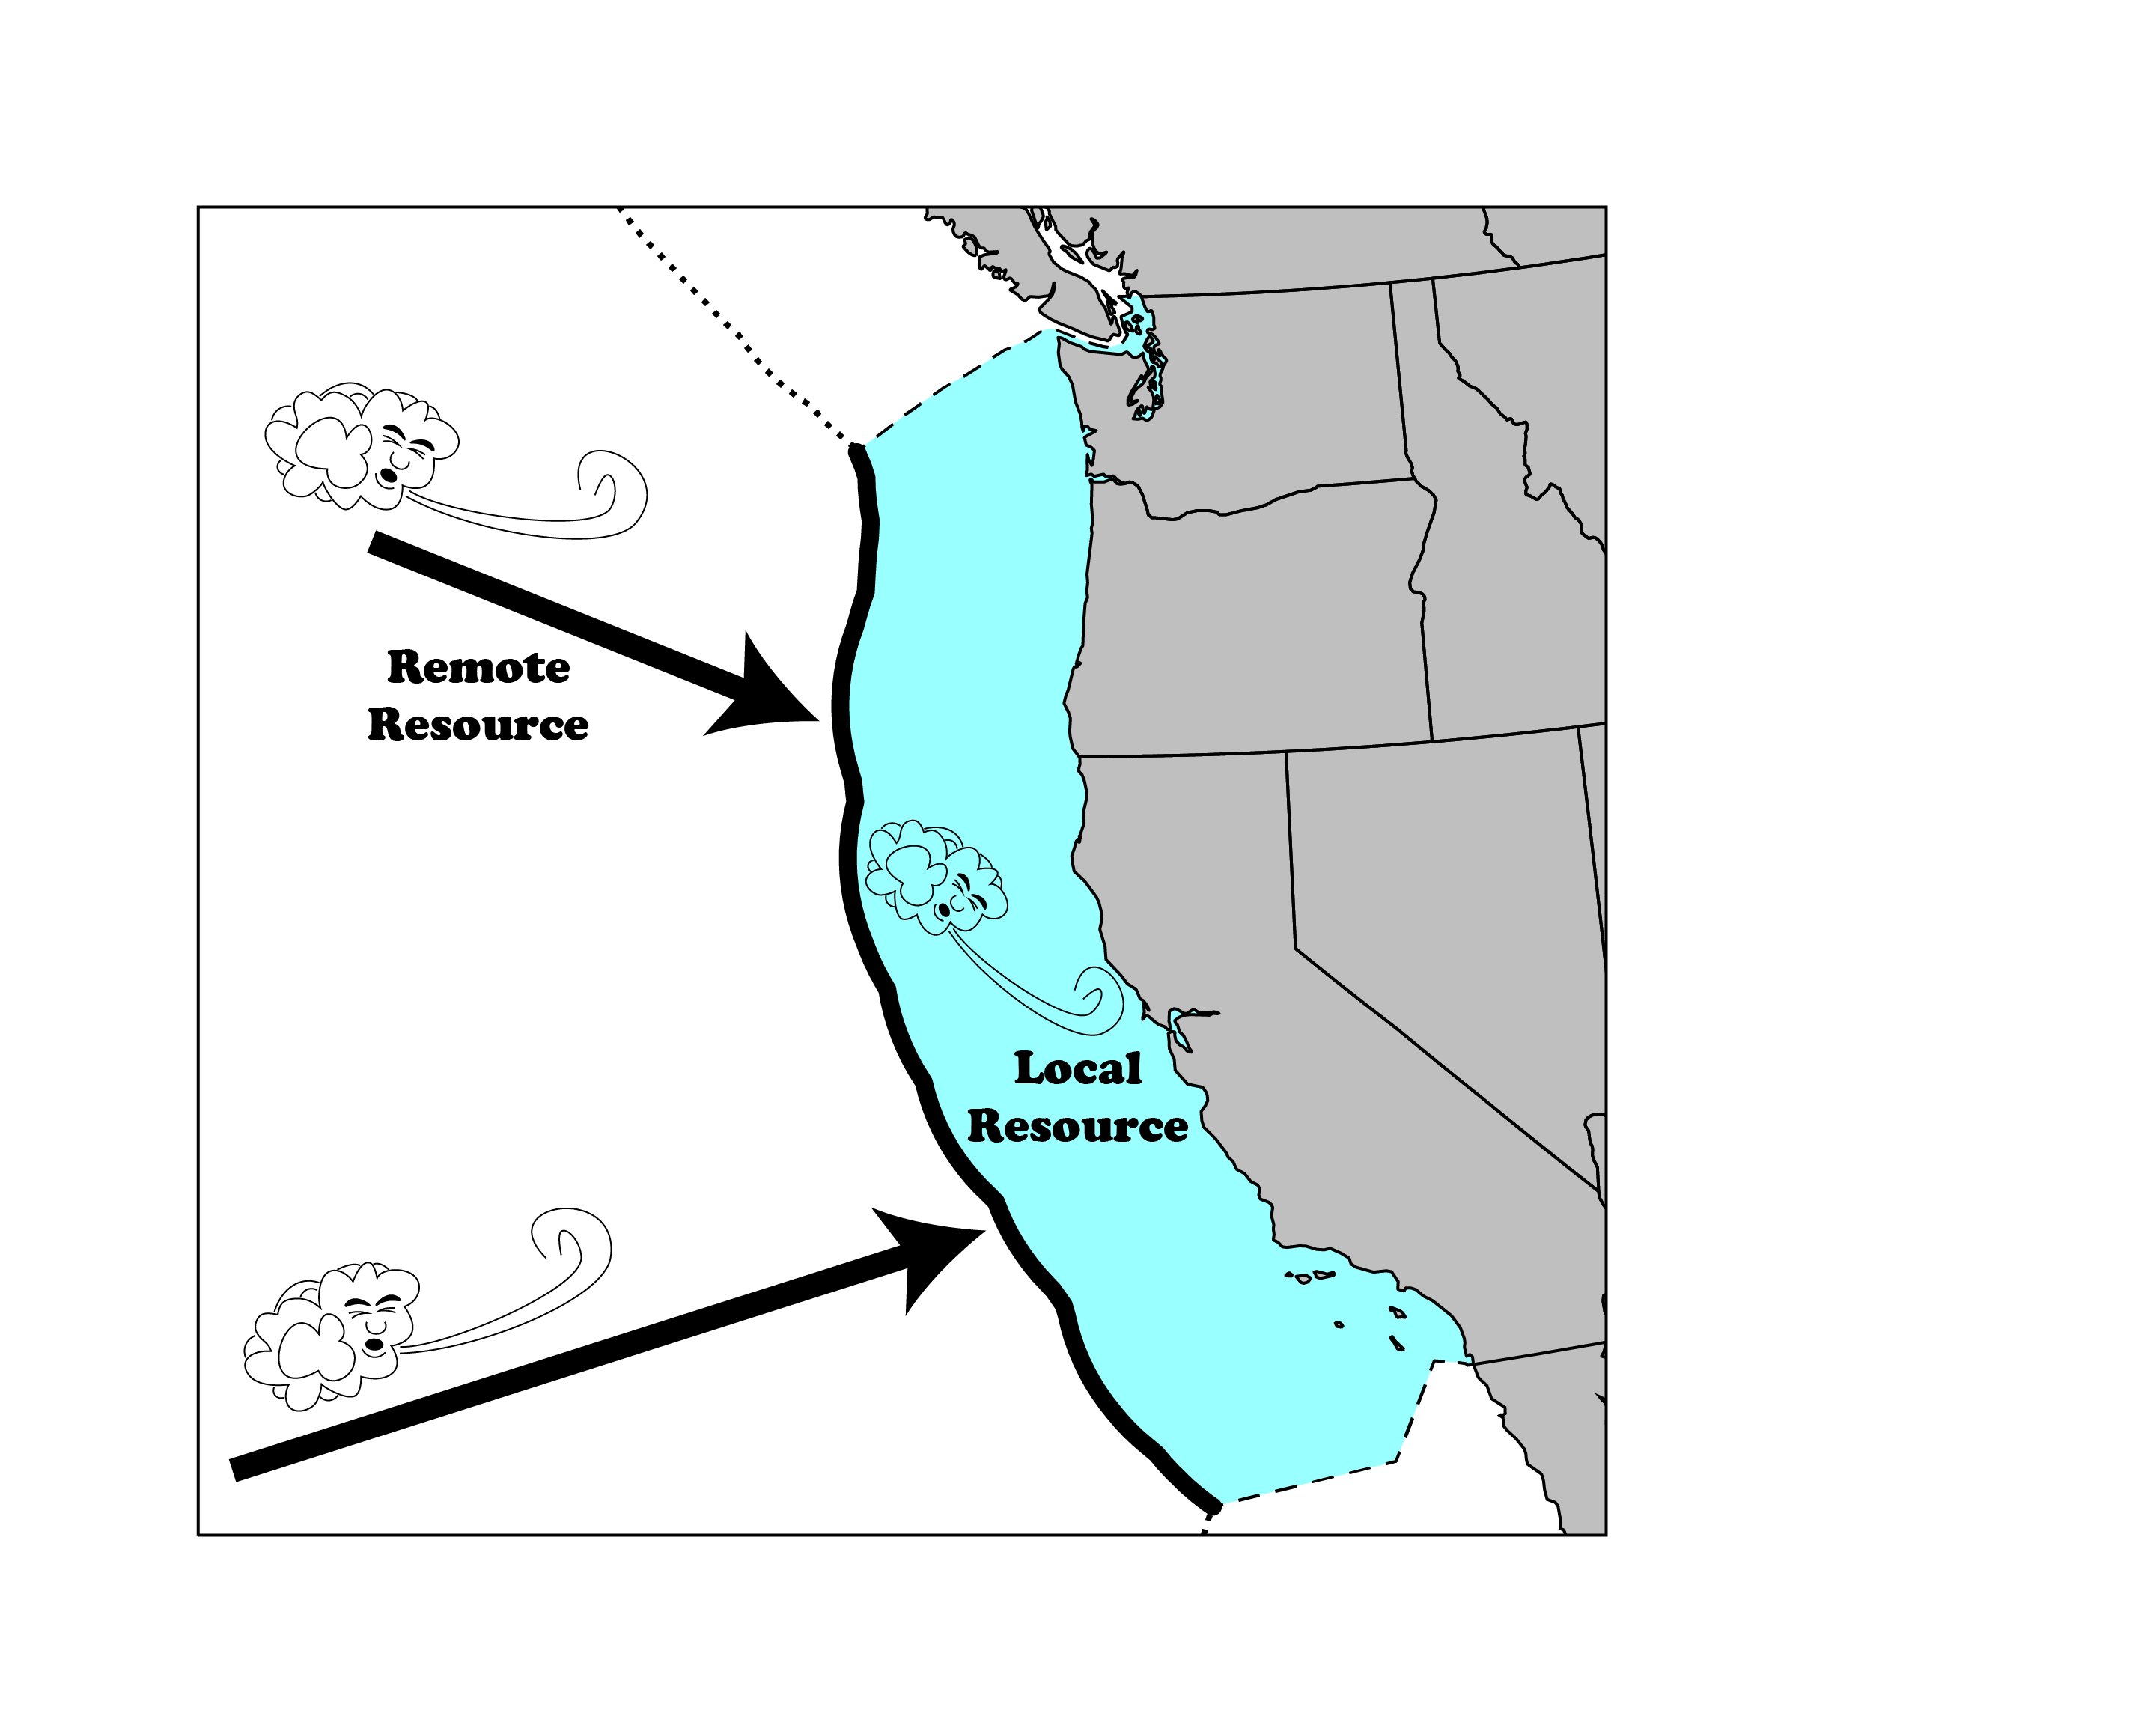
\includegraphics[width=0.9\linewidth]{../diagram/EEZ_contour03_edit01.png}
  \caption{A diagram depicting the U.S. West Coast’s ‘remote’ (arrows) and ‘local’ (cyan region) resource.}
  \label{fig:diagram:west-eez}
\end{figure}

A secondary objective of this work is to provide a refined estimate of the U.S. wave resource based on this new method, and new model results. A tertiary objective is to provide guidance that helps address limitations in site assessment, which we hope will eventually lead to a unified methodology for site and regional wave resource assessment.

These objectives are accomplished by first discussing the details of regional assessments (section 2), and then presenting our proposed approach (section 3). In section 4, we present the results of this approach applied to each region of the U.S. coastline in comparison to alternate methods that have been used. Section 5 provides a detailed discussion of the results, including a justification for the proposed approach, and a summary of how the proposed approach can be applied in different scenarios. We conclude with a summary of results, the proposed methodology, and a view toward how to unify wave energy site and resource assessment
% Need to define `theoretical resource assessment'

This paper has two primary objectives: 1) to define a new methodology for quantifying theoretical wave resource that addresses critiques of previous approaches that can be applied at any scale, and 2) to apply that method to all U.S. regions to obtain an updated assessment of the nation's wave energy potential (theoretical resource).

%%% Local Variables:
%%% TeX-master: "wave_res"
%%% End:

%\section{Background}

\section{Method} \label{sec:method}

\begin{figure}[ht]
  \centering
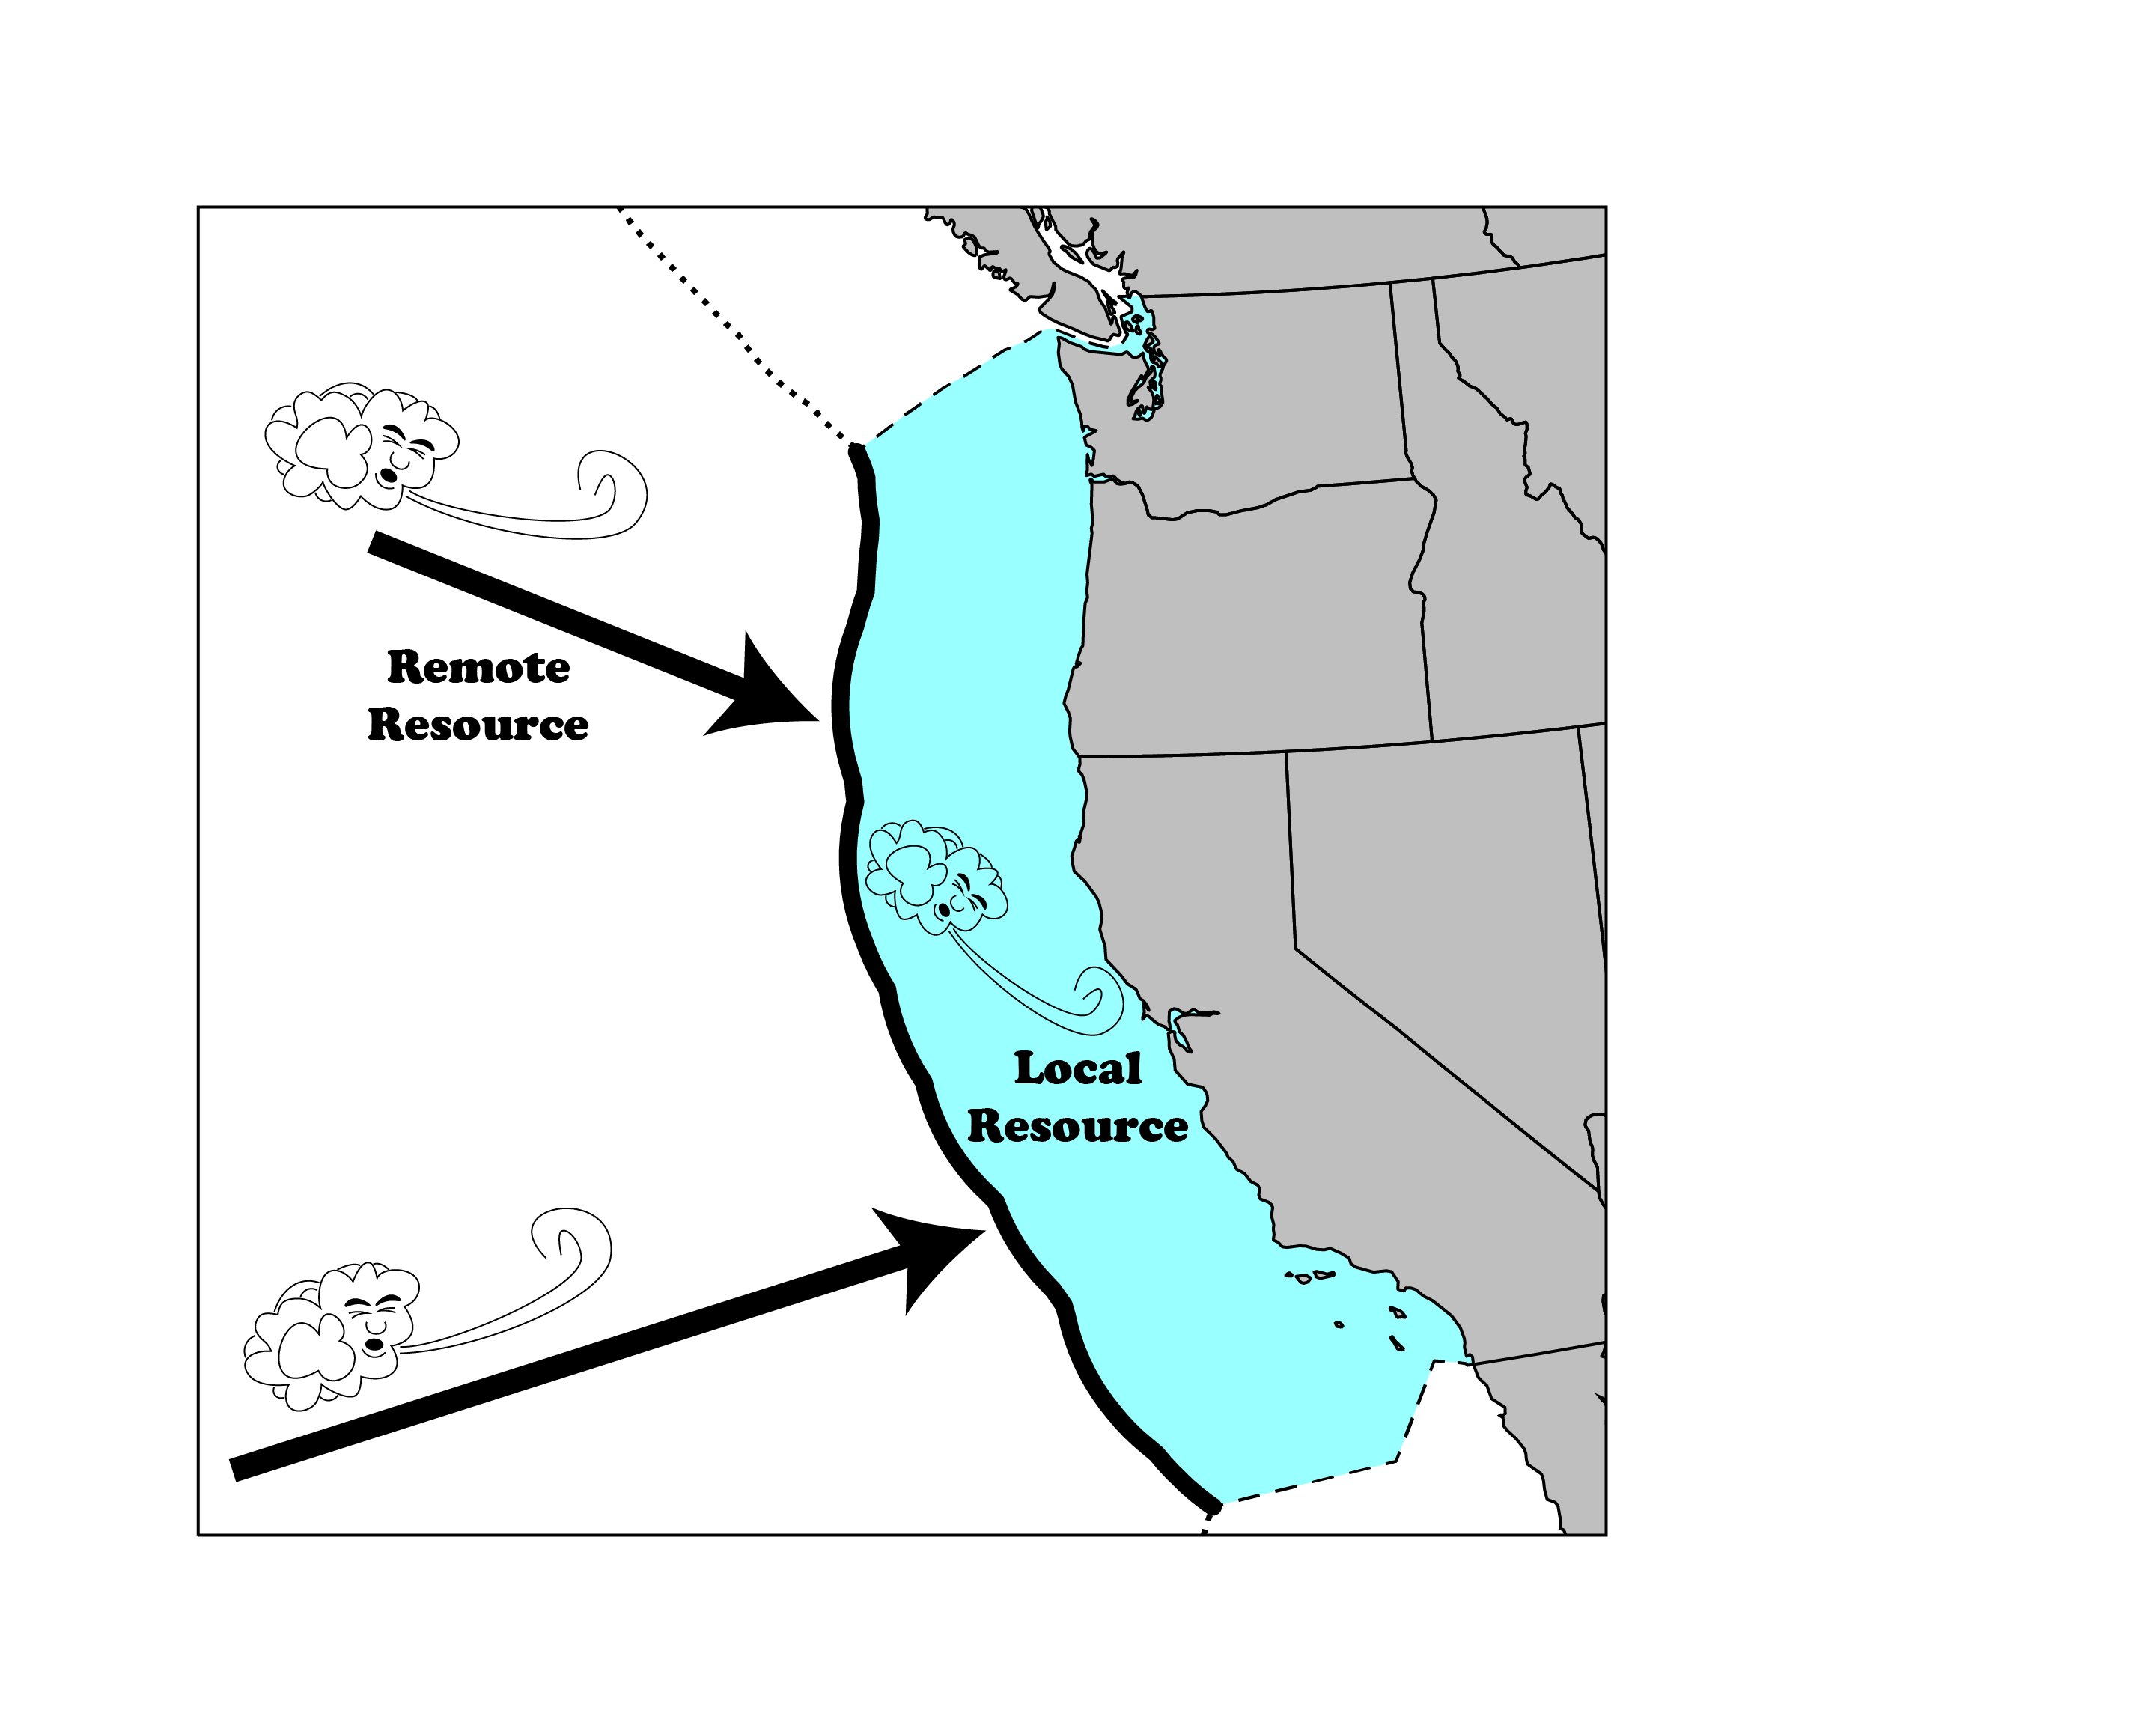
\includegraphics[width=0.9\linewidth]{../diagram/EEZ_contour03_edit01.png}
  \caption{A diagram depicting the U.S. West Coast’s ‘remote’ (arrows) and ‘local’ (cyan region) resource.}
  \label{fig:diagram:west-eez}
\end{figure}

The overarching goal of this study is to develop an accurate methodology for estimating the total theoretically available wave resource for a given region. The methodology has been formulated to address outstanding critiques of earlier works, namely: the method should eliminate or at least minimize ``double counting'', and it should also include all sources of wave energy that are legitimately a portion of the region's resource. With these objectives in mind, we propose that regional resource assessment should be conducted according to the following principles:

\begin{enumerate}
\item {\bf Follow IEC TS-101 standards for numerical model setup, configuration, and validation.} The IEC standards have done an excellent job of describing detailed guidelines for model setup and procedures for validation. We have followed the ``Class 1, Reconnassance" level here \note{RIGHT?!, or did we follow class 2?, ... or did we not follow IEC?!}, and it is most likely the most relevant class for other regional assessments, but there may be cases where it is desirable to follow class 2 or 3. One thing that should be added to the IEC guidance is the model must be configured to output the source terms, so that the `local resource' (below) can be computed.
\item {\bf The total resource is the sum of the remote and local resource} (Figure \ref{fig:diagram:west-eez}). The majority of existing wave resource assessments have considered the remote resource only. The inclusion of the local resource is a means for accounting for the 'recovery' of the wave-field downstream of where energy is extracted.
\begin{itemize}
    \item {\bf Calculate the ``remote resource'' utilizing a one-way dot-product at the boundary of the domain.} This approach has been used in several previous wave resource assessments \citep{gunnQuantifyingGlobalWave2012, hemerRevisedAssessmentAustralia2017}. This is a fundamental component of wave resource assessment because it avoids the {\em double} counting inherent in the `unit-circle' method used in EPRI 2011, and also avoids {\em under} counting that can occur when using a traditional dot-product. A detailed investigation of the importance of this approach can be found in Appendix \ref{appendix:one-way-method}.
    \item {\bf Include the local wave generation:} this consists of quantifying the wave resource generated landward of the boundary. Considering this part will provide a complete quantification of the resource. Estimates of the resource generated locally has implications to estimating the wave recovery potential, should a significant amount of wave energy be harvested. To the authors' knowledge this has not been considered in previous resource assessments.
\end{itemize}
\item {\bf Extend the assessment to the edge of the region's legal boundaries.} Based on Article 56 of the U.N. Law of the Sea — which states that "in the exclusive economic zone, the coastal State has sovereign rights [to] the production of energy from the water, currents and winds" — we propose that national resource assessments should utilize the EEZ as the domain over which wave energy resource totals are calculated \citep{unitednationsgeneralassemblyConventionLawSea1982}. Furthermore, the sum of the resource computed for two regions independently should be the same as if the resource is computed for both regions combined. In particular, this means that the method should not count wave energy fluxing across the boundary between the two regions.
\end{enumerate}

\subsection{Numerical Model} \label{sec:method:model}

Wave resource assessments typically rely on the use of wave model `hindcasts' to estimate the history of the wave field over the region(s) of interest, and then to compute estimates of the theoretical resource from the model output. The reason for this is that in-situ or remote measurements do not cover the oceans with enough resolution, spatially and temporally, to characterize the spatial variations of waves that occur at short scales. 
In this work all wave climate hindcasts are simulated using WAVEWATCH III\textregistered v5.16 \citep{tolmanDistributedmemoryConceptsWave2002,tolmanwavewatch}.

WAVEWATCH III\textregistered (hereafter WW3) is a  well established numerical model that has been implemented successfully in many previous wave resource assessments \citep[e.g.,][]{garcia-medinaWaveResourceAssessment2014,hemerRevisedAssessmentAustralia2017,yangWaveModelTest2017}.
WW3 solves the five-dimensional action balance equation:

\begin{align}
  \frac{d N}{d t} = \frac{\Src{tot}}{\sigma} = \frac{1}{\sigma}\left ( \Src{in} + \Src{ds} + \Src{brk} + \Src{nl} + \Src{bot} \right )
  \label{eqn:actionbalance}
\end{align}
where $N(t,x,y,\sigma,\theta) \equiv D/\sigma$ is the wave action, $D$ is the variance spectrum, $t$ is time, $x$ and $y$ are the spatial coordinates, $\sigma$ is the radian frequency, and $\theta$ is the direction of wave propagation.
The wave action is conserved in the absence of sinks and sources of energy, their combined effect is represented as $\Src{tot}$.
The models do not include ocean currents so that $\sigma$ (intrinstic frequency) is spatially constant, and therefore wave energy (i.e., variance, $D$) is a conserved quantity (i.e., energy is only gained or lost by the source terms above).

In this study we implement the ``ST4'' physics package option in WW3 to simulate wind energy input ($\Src{in}$) and dissipation due to whitecapping ($\Src{ds}$) \citep{ardhuinObservationSwellDissipation2009}.
The wind forcing (for both the global and regional domains) is taken from NOAA's Climate Forecast System Reanalysis (CFSR) \citep{sahaNCEPClimateForecast2010}. The non-linear quadruplet interactions ($\Src{nl}$) are modeled with the Hasselmann and Hasselmann (\citeyear{hasselmannComputationsParameterizationsNonlinear1985}) formulation. Bottom friction ($\Src{bot}$) and depth induced wave breaking ($\Src{brk}$) are modeled with the JONSWAP Hasselmann etal. \citeyear{hasselmannMeasurementsWindwaveGrowth1973} and Battjes and Janssen \citeyear{battjesEnergyLossSetup1978} models, respectively. Finally, the effect of sea ice is considered by using a time varying mask based on the ice coverage fields from CFSR. Default parameters are used for all formulations.

The WW3 simulations span a 32-year period from January 1, 1979 to December 31, 2010. The first year (1979) is treated as a 'spin-up' year, and is not included in any calculations of resource totals. Variability in the wave climate on timescales longer than the 31-year period included in the average are not considered (i.e., changes in the wave resource due to climate change are not included). The wave spectrum is discretized with 24 equally spaced bins in $\theta$ space and 29 logarithmically spaced frequency bins from 0.035Hz to 0.5Hz with an increment factor of 1.1. 

Model grids and bathymetry come from the NOAA NCEP hindcast Phase 1 mosaic-model \citep{chawla2011wavewatch,chawla201230}. In this system a global model (0.5$^{\circ}$ resolution) drives regional models (10" - 4" resolution) providing complete coverage over the U.S. EEZ with higher resolution focused on shallower waters. This model was reimplemented to store wave spectra and source terms at a high resolution.

Model output is collected at the U.S. EEZ around Alaska (excluding the Arctic Coast), Atlantic Coast, Caribbean Coast (Puerto Rico and U.S. Virgin Islands), Gulf Coast, Hawaii (excluding the Papah$\bar{\text{a}}$naumoku$\bar{\text{a}}$kea Marine National Monument), and the West Coast. Full variance spectra are stored at the U.S. EEZ boundary (at 200 nmi from shore, and along EEZ `borders' with other nation's). Inside the EEZ, directionally integrated source term output is collected at lines of equal distance from shore from 18.5 km (10 nmi) to 351.9 km (190 nmi) every 18.5 kms. Both output types are collected at hourly intervals every 1/6$^{\circ}$ along the defined lines.

This model configuration is mostly aligned with the IEC TS 62600-101 requirements for a reconnaissance class resource assessment. The requirements for physical processes are met with the exception of the inclusion of wave-current interactions and the effect of tides. It is not expected that the tides will influence waves significantly beyond 18.5 km from shore. Wave-current interactions can be important particularly around the Gulf Stream, thus the exclusion of this must be revisited in future studies. The numerical requirements from IEC TS 62600-101 indicate that spherical coordinates must be used with a minimum temporal resolution of 3h, 25 wave frequency components, 24 azimuthal directions, and a minimum spatial resolution of 5 km. All but the latter are met in this study, the regional models at 4" have a meridional resolution of 7.4 km.

In WW3, as it is customary in third-generation spectral wave models, the waves are computed over a specified spectral width after which a spectral tail is appended to represent the energy in the high frequencies \citep[e.g.][]{ardhuinObservationSwellDissipation2009}. This frequency cutoff is generally the minimum of the highest described frequency and the cutoff supported by the source term formulations. The simulations in this study are performed with the default high frequency cutoff:

\begin{align}
  f_{c} = \frac{2.5}{T_{m01}}
\end{align}
where $T_{m01}$ is the mean spectral period. The source term integrals are performed for the range where the wave spectrum is actively simulated.

\subsection{Calculate Resource Totals} \label{sec:method:calc}

In this work we propose that the total theoretical wave resource, $R_T$, be defined as a sum of `remote' and `local' components:
\begin{align}
  R_T = R_R + R_L
\end{align}
The remote resource, $R_R$, is the piece of the wave energy resource that has previously been defined as the total wave resource \citep{gunnQuantifyingGlobalWave2012,EPRIwaveresource2011}, while the local resource, $R_L$, has not previously been included in wave resource assessments.

\subsubsection{Remote Resource} \label{sec:method:calc:remote}

The remote resource is computed as a line-integral of the wave energy that fluxes toward the coastline across the EEZ boundary when it is bordered by international waters. 

\begin{align}
  R_R = \rho g \int_{\ell}\iint \delta \, c_g(f) \, \bar{D}(f,\theta) \d f \d \theta \d l
\label{eqn:RR}
\end{align}
Where $c_g(f)$ is the wave group velocity, $\ell$ is the integration contour, and $\delta$ is the directionality coefficient which we take to be $\delta = \cos(\theta_n - \theta)$ for waves propagating toward the coastline, and $\delta = 0$ otherwise. 
$\theta_n$ is the direction normal to the contour pointing toward the shoreline. 
This `one-way' condition ensures that waves propagating offshore are not {\em subtracted} from the total \citep[]{gunnQuantifyingGlobalWave2012}. A detailed rationale for the one-way approach is included in appendix \ref{appendix:one-way-method}. The over-bar denotes a time-average of the wave-variance spectrum over the 31-year period from Jan. 1 1980, through Dec 31, 2010.

In this work, the integration contour $\ell$ is the segments of the U.S. EEZ that separate U.S. EEZ waters from the open-ocean (hereafter the `EEZ boundary'; thick black line in Figure \ref{fig:diagram:west-eez}), and does not include the EEZ segments that separate one nation's EEZ from that of a neighbor (hereafter the `EEZ borders'; thin dashed lines) \citep[]{flandersmarineinstituteMaritimeBoundariesGeodatabase2018}. This is because wave-energy that fluxes across EEZ borders will be counted -- using the methodology described here -- by the nation from which that resource originated. For example, waves that propagate southward across the Canada-U.S. EEZ border are counted as Canada's resource, and waves that propagate northward across this border are counted as U.S. resource. Either way, these waves will already have been counted in the originating nation's resource, and so including wave fluxes across these borders would only lead to `double counting'.


\subsubsection{Local Resource} \label{sec:method:calc:local}

While neglecting the local resource may be reasonable for small projects, the fact that it
typically has been implicitly ignored has raised legitimate questions about the validity of the methodologies, which has led to skepticism and confusion. The local resource is computed as an area-integral of all wave source- and sink-terms, except for bottom friction:

\begin{align}
  R_L &= \rho g \int_{EEZ}\iint \left ( \bar{S}_{in} + \bar{S}_{ds} + \bar{S}_{nl} \right ) \d f \d \theta \d A
\label{eqn:RL}
\end{align}
where $dA$ is differential-area integral of the source terms. Since the model results are output in spherical coordinate system, the coordinates were transformed using an Albers equal area projection before performing the area integral. By performing these projections on a region-by-region basis with carefully chosen projection parameters, this approach introduces $<1\% $ local distortion at the edges of the largest regions (Alaska), and therefore introduces a $\ll 1\%$ error in the total estimate of $R_L$.

\paragraph{Discussion of the terms included in $R_L$}

Note that the depth-induced wave breaking ($S_{brk}$) and bottom friction ($S_{bot}$) terms from \eqref{eqn:actionbalance} are neglected in \eqref{eqn:RL}.
The $S_{brk}$ term is neglected because this term closes \eqref{eqn:actionbalance} by dissipating all \note{(or nearly all? is energy ever reflected?)} of the energy that arrives at the shoreline. Including this term, therefore, would negate all energy arriving from offshore (i.e., in $R_R$ and $R_L$). This is precisely contrary to the purpose of wave energy resource assessment, because the purpose of wave energy technology is to capture wave energy {\it before} it dissipates at the shoreline. The $S_{bot}$ term is neglected for similar reasons: in deep water it is negligible, and so we assume that wave energy can be extracted before this term becomes relevant. For example, even along the U.S. East Coast and in the Gulf of Mexico -- where coastal waters are relatively shallow -- the EEZ spatial-average of $S_{bot}$ is three orders of magnitude smaller than that of $S_in$.

It should be noted that the white-capping term ($\bar{S}_{ds}$) is negative, and the non-linear term ($\bar{S}_{nl}$) -- which transfers energy from high- to low-frequency -- is negative on average (i.e., across frequency and time) \note{Is the integral in frequency of this term always negative? Suggestions about how to say "this term is negative" more clearly?}. 
Based on these facts, it is tempting to assume that wave energy originating from the large positive term $S_{in}$ could be absorbed prior to these other terms dissipating it because this approach would yield a significantly larger local resource. While that approach would yield a significantly larger local resource, doing so is scientifically questionable for several reasons. First, the spatial and temporal scales at which $S_{in}$ delivers energy to the wave field is similar to the scales at which $S_{ds}$ removes it. In other words, significant white-capping and dissipation occurs when winds generate waves.

Second, the details of wave-generation is an active area of research, with large uncertainty associated with each term's magnitude \citep[e.g.,][]{garcia-medinaWaveResourceAssessment2014}. The sum of the terms, on the other hand, is relatively well constrained as demonstrated by the performance of wave models in general (i.e., via wave-model validation studies \note{NEED CITATIONS}). Third, there are significant practical questions about extracting small-wave energy (i.e., at the scales that the majority of $S_{in}$ energy exists) across sufficiently large spatial-area for the energy to be sizable. Therefore, it makes sense to include the $S_{nl}$ term in order to properly quantify the degree to which low-frequency waves are generated by winds.

There is certainly an inherent tension here between, ``including the local resource in order to provide a complete assessment of the {\em theoretical} wave resource'', and assuming that some pieces of the wave source terms (wind input) are inaccessible on {\em practical} and {\em technical} feasibility grounds. In other words, some might argue that including the negative source terms belongs in a technical or practical resource assessment. However, we argue that including $R_L$ as defined here is already a relatively optimistic proposal. 
The task of quantifying any resource, including the theoretical resource, involves making some assumptions about what is realistic and what is not. 
Perhaps more importantly, until we have a better understanding of the magnitude (i.e., uncertainty) of the individual terms, and we have technologies that show promise for extracting high-frequency energy at spatial and temporal scales between wind-input and non-linear transformation to lower frequency, neglecting these negative terms seems scientifically dubious.

\paragraph{Discussion on methodological changes related to $R_L$}
\textcolor{blue}{Not sure about the organization of this subsection. Right now it feels like a hodge-podge of miscellaneous items.}

This piece has not typically been considered in wave resource assessments. This is most likely because it is obvious that for projects within 10 to 20 miles of shore - where it seems reasonable to assume the majority of projects will be for the next several decades - $R_L \ll R_R$. However, when we are taking the perspective of an assessment of the nation's resource - which according to the U.N. law of the sea legally extends to the edge of the U.S. EEZ - $R_L$ is an important piece of the total energy available. By accounting for this term, this methodology directly incorporates the energy added to the wave field over that area. While it does not directly address the question ``how quickly will the wave-field re-energize down-wave from a wave farm?'' It does explicitly include this energy. \textcolor{blue}{Still not happy with this paragraph. What am I trying to say here?}

However, because the source terms in \eqref{eqn:RL} depend on the sea-state and the sea-state depends on energy extracted ``up-wave'', there is ambiguity in estimating $R_L$ related to where and when wave energy is extracted by WECs. To address this, we calculate two estimates of $R_L$. The first, `natural local resource' ($R_{L_\circ}$) is calculated from the source-terms where waves from the global domain propagate freely throughout the regional domain (the EEZ). The second, `potential local resource' ($R_{L_*}$) is calculated from the source-terms when no wave energy propagates across the EEZ boundary. In other words, this is a `lake case' that only contains waves generated by winds within the regional domain.

In all cases we examined, $R_{L_*}$ was found to be greater than $R_{L_\circ}$ (see Appendix \ref{appendix:flux-vs-area} for details). In the sense that $R_L$ is meant to be an estimate of the maximum energy available, this suggests that $R_L$ could be defined as being equal to $R_{L_*}$. However, the scenario of removing all wave energy from the wave field at the edge of the EEZ is so hypothetical that it seems unrealistic to use this value to define $R_L$. Therefore, we choose to treat these two estimates of $R_L$ as an uncertainty range for the value.

It is worth noting that -- though a line-integral that accounts for directionality of the wave flux (a {\em vector quantity}) is applicable for estimating $R_R$ \eqref{eqn:RR} -- directionality is {\em not } important to estimating $R_L$ correctly in \eqref{eqn:RL} (i.e., all directions are weighted equally). This is because the source terms are {\em scalar quantities} that are functions of direction per unit-area, and therefore an area-integral applies.
%This can be understood by considering the hypothetical case of an array of WECs that covers the entire EEZ. The wave energy that is added locally within the EEZ will be absorbed -- regardless of it's direction -- by the array before it reaches the edge of the EEZ where a line-integral would be appropriate (i.e., when directionality is important).


\subsection{Methodological differences with EPRI 2011}
\label{sec:method:changes}

Before proceeding to the results, we take a moment to briefly describe four major methodological differences between this work and EPRI 2011. First, we have utilized updated models \note{GGM: can you describe briefly the major changes here? Probably just a sentence or two?} Second, we utilize a one-way dot-product, where EPRI 2011 used the ``unit-circle'' method which the National Academy noted would cause double-counting. Third, we include the local resource, $R_L$, in the total. Finally, we extend the analysis to the edge of the EEZ (200 nautical miles from shore), where EPRI 2011 nominally used the 200 meter isobath, or a 50 nautical miles from shore line, depending on the region.

%%% Local Variables:
%%% TeX-master: "wave_res"
%%% End:

\section{Wave Energy Resources of the United States}
\label{sec:results}

We estimate the total U.S. Resource to be 3300 TWh/yr, with an additional 790 TWh/yr available in the potential resource (Table~\ref{table:totals}). This is an increase of  25\% compared to earlier DOE wave resource assessments. This result, however, should not be interpreted as an indication of a growing resource (e.g., due to climate change). Instead, the increase is due to a more complete accounting of wave energy sources (i.e., the ``local resource''), and from extending the domain to include the entire U.S. EEZ. Wave energy has consistent seasonal cycle across all regions: it is a late-fall and winter dominated resource (Figure \ref{fig:annual-cycle}), with a peak in December or January and a minimum in summer.

The inter-annual variability of the resource — depicted by box-plots for the West Coast in Figure \ref{fig:annual-cycle}) but with consistent results across regions — is generally proportional to the resource amplitude: low variability in summer and high-variability in winter. During energetic winter months, the monthly-averaged resource can vary by more than 50\%, but in general the inter-annual variability is less than 30\% of the month's mean. This suggests that during energetic winter months wave energy projects should be expected to deliver at least their annual mean, with the potential to provide up to three times that.

Including the potential resource (thin lines in Figure \ref{fig:remote-freq}) in the spectral distribution shifts the distribution to higher frequency, and adds a short-period (high-frequency) peak at 2 to 4 seconds compared to the remote only resource (thick lines). This is the influence of the wind input terms, which tend to add energy at high-frequency. The effect is essentially the same when adding the natural local resource (not shown). The low-period (high-frequency) energy contained in the local resource has not typically been of interest to the WEC community, but as interest in PBE markets grow - especially those involving small WECs for low power applications - there may be more interest in this portion of the wave energy spectrum.

\subsection{The U.S. West Coast}

The west coast is a promising region for wave energy because it possesses a large theoretical resource (510 TWh/yr, table \ref{table:totals}) and has the coastal population density to make use of it. The inner-shelf resource (410~TWh/yr, table \ref{table:totals}) is equal to ~40\% of the electricity consumption of California, Oregon, and Washington (2018 total: 943 TWh/yr), which suggests that there is sufficient resource to play a sizable role in the region's energy profile in the foreseeable future \citep{energyinformationadministrationStateEnergyConsumption2020}. The resource along the northern half of the west coast — Oregon, Washington, and Northern California — is particularly energetic: the annual-average wave energy flux exceeds 40 kW/m in several places.

This resource is composed primarily of long-period waves — 90\% of the resource is contained between 6.5 and 19 seconds (Figure \ref{fig:remote-freq}) — which carry more energy per-unit of wave amplitude. These waves arrive at the shoreline from throughout the Pacific basin \citep{perezESTELAMethodEvaluating2014}. The PacWave test site, offshore of central Oregon, has been created to be the first U.S. "grid-connected full-scale test facility", is critical to testing wave technologies and demonstrating that they can perform efficiently and reliably in this world-class fully-energetic environment where winter storms regularly deliver wave more than 8 meters in amplitude \citep[e.g.][]{allan_climate_2006}.


\subsection{The U.S. East Coast}

The east coast also possesses a sizable wave energy resource (290 TWh/yr), but it is composed primarily of the local resource (180 TWh/yr). This is because mid-latitude westerly winds tend to generate wave energy that propagates eastward and builds to a sizable resource across the broad fetch of the U.S. EEZ. Relatively less wave energy — compared to the West Coast at least — from the open Atlantic propagates onshore toward the U.S. eastern coastline (compared to the U.S. west coast). The remote resource, therefore, is relatively modest (110 TWh/yr at the EEZ, and 90 TWh/yr on the inner-shelf). Because this resource is dominated by waves that are generated locally, the waves tend to be much shorter-period (90\% of the energy is between 6 and 15 seconds, Figure \ref{fig:remote-freq}).

The offshore directed winds cause the most energetic wave resource to be located near the edge of the EEZ offshore of New England (Figure~\ref{fig:maps}). Note here that the omni-directional wave power shows the combined effect of local and remote resource. The east coast inner-shelf resource is somewhat smaller than the EEZ remote resource because a fraction of energy in these westward-propagating remote waves are dissipated by whitecapping from the westerly winds.

While the East Coast wave resource is modest in comparison to the West Coast, it is too early to neglect the potential for wave energy here. As wave technologies continues to mature and if the cost of the technology is low enough, sites and regions previously considered uneconomical may prove to be attractive, especially in markets where energy prices are already high and alternate renewable sources are limited or constrained. 

\subsection{Hawaii}

Hawaii also possesses a large resource (380 TWh/yr) composed primarily of waves propagating southward from the North Pacific. The local resource is relatively small (10 TWh/yr), due primarily to the fact that the sea-state in this region is -- in the long-average perspective of regional resource assessment -- approximately `steady-state' because the wind input and dissipation are nearly in balance. The inner-shelf Hawaiian resource (120 TWh/yr) is smaller than the EEZ remote resource because the the 10 nautical-mile boundary is a much ``smaller net'' in comparison to the full EEZ.

Hawaii is a particularly interesting case because the resource is large compared to the State's electricity consumption (26 TWh/yr), and because energy-prices are high. Wave energy may be particularly valued in Hawaii where space is limited for land-based renewable alternatives; and the tourist economy may especially value WECs with limited surface expression. Together, these factors make Hawaii a likely early-market for wave energy technology. The Navy's Wave Energy Test Site on the north shore of Oahu, is supporting the development and demonstration of technologies for meeting the potential demand \citep{crossEarlyResearchEfforts2015}.

The Hawaiian resource is bi-modal with a peak at 14 seconds and a peak at 9 seconds. This ``double-peak'' is primarily a seasonal effect where waves with period 11-12 seconds are more prevalent in January and February, while waves with period 8-10 seconds arrive in March and April \citep[][]{stopa2013wave}. 

\subsection{Alaska}

Nearly two-thirds of the nation's wave energy resource is in Alaska (2000 TWh/yr), split approximately evenly between the remote and local pieces. However, the majority of this resource is `stranded' very far from markets large enough to utilize more than a few MW of power. Still, if the cost of large-scale energy storage technologies become sufficiently economical (e.g., renewable fuels, batteries, etc.), or if energy-intensive industrial activity were sited in this region, this wave resource could become valuable. In the shorter-term, the villages along Alaska's coastline -- where energy prices are very high -- represent an opportunity to demonstrate commercial viability before scaling the technology up \cite{alaskaenergyauthority2019PowerCost2020}. Or this energy could be used in-place for Blue Economy applications such as charging batteries on vessels or for scientific instruments during long transits or exploration. 

\subsection{Gulf of Mexico, Puerto Rico, and U.S. Virgin Islands}

The Gulf of Mexico's wave resource is rather small, composed almost exclusively of locally-generated, short-period waves.  The wide shelf in this region also has the effect of damping out any waves that are generated. The presence of hurricanes in this region confounds the challenge of developing wave energy technologies for this region because devices would need to be designed to survive the extreme conditions that come with hurricanes. The same basic conclusions can also be drawn for Puerto Rico and the U.S. Virgin Islands. Throughout the Gulf and these islands there may be niche applications, or specific sites, where wave energy can be utilized. But it seems unlikely that utility-scale wave power will contribute significantly to the power needs.


%\begin{table}[ht]
%  \centering
%  \begin{tabular}{|c|c|c|c|c|c|}
%    %\cline{2-7}
%    %%\multirow{1}{*}{Region}
%    %\multicolumn{1}{c|}{} & {\it EPRI 2011} & \multicolumn{5}{c|}{New} \\
%    \hline
%    Region & Inner-Shelf & Remote & \multicolumn{2}{c|}{Local} & Total \\
%    & & & Natural & {\it Potential} & \\
%    \hline
%    Alaska & 1190 & 1040 & 990 & {\it 1510} & 2030 {\it – 2550} \\
%    West Coast & 410 & 420 & 90 & {\it 210} & 510 {\it – 630} \\
%    Hawaii & 120 & 370 & 10 & {\it 100} & 380 {\it – 470} \\
%    East Coast & 90 & 110 & 180 & {\it 230} & 290 {\it – 340} \\
%    Gulf of Mexico & 20 & 13 & 56 & {\it 57} & 69 {\it – 70} \\
%    P.R. \& U.S.V.I. & 20 & 6 & 11 & {\it 27} & 17 {\it – 33} \\
%    \hline \hline
%U.S. TOTAL & 1850 & 1960 & 1340 & 2130 & 3300 {\it – 4090} \\
%\hline
%  \end{tabular}
%  \caption{Wave resource assessment results by region and totaled for the entire U.S. (all values in TWh/yr). The range in %the "Total" column indicates the sum of Remote + Local (lower value) and Remote + Potential (higher value, in italics).
%  \noteSelf{Do we need to be more careful w/ significant digits here?}
%  }
%  \label{table:totals}
%\end{table}



\begin{table}[ht]
  \centering
  \begin{tabular}{|c|c|c|c|c|}
    %\cline{2-7}
    %%\multirow{1}{*}{Region}
    %\multicolumn{1}{c|}{} & {\it EPRI 2011} & \multicolumn{5}{c|}{New} \\
    \hline
    Region & Inner-Shelf & Remote & Total & Potential \\
    \hline
    Alaska & 1200 & 1000 & 2000 & +520 \\
    West Coast & 410 & 420 & 510 & +120 \\
    Hawaii & 120 & 370 & 380 & +90 \\
    East Coast & 90 & 110 & 290 & +50 \\
    Gulf of Mexico & 20 & 13 & 69 & +1 \\
    P.R. \& U.S.V.I. & 20 & 6 & 17 & +16 \\
    \hline \hline
    U.S. Total & 1900 & 2000 & 3300 & +790 \\
    \hline
  \end{tabular}
  \caption{Theoretical wave resource results by region and totaled for the entire U.S. (all values in TWh/yr). The inner-shelf resource is the remote resource 10-nautical-miles from shore. The total is the sum of the local and remote resource, and the potential is how much additional energy is available if the entirety of the remote resource is removed at the EEZ boundary. All values are reported to two significant figures, therefore totals may not equal sum of regional values.
  }
  \label{table:totals}
\end{table}



\begin{figure}[ht]
  \centering
  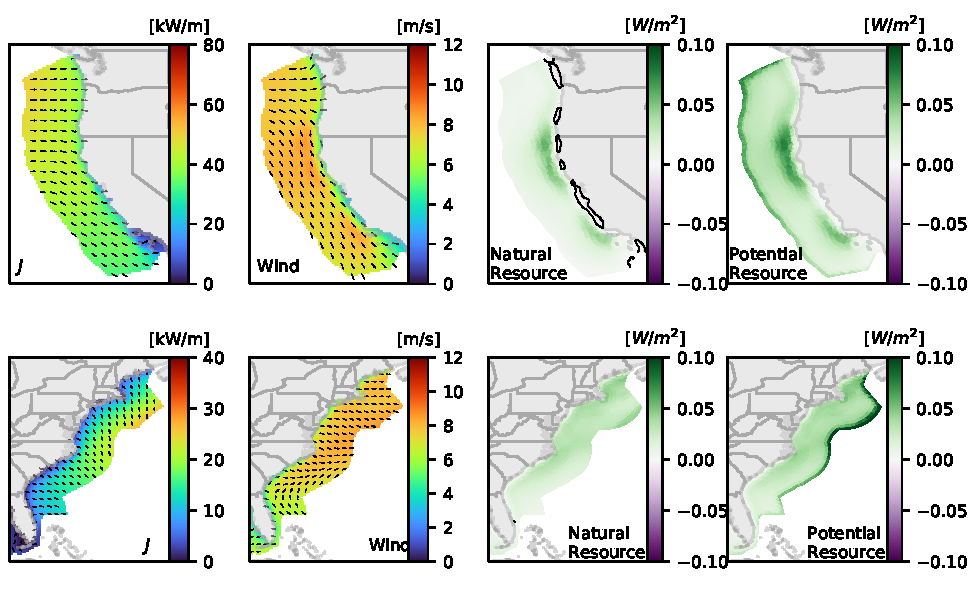
\includegraphics[width=\textwidth]{../fig/Yearly_spatial_seasonal_mag_6.pdf}
  \caption{Maps of average omnidirectional wave power (left), wind (second column), natural resource (third column), and potential resource (roth) for the West Coast (top) and Atlantic Coast (bottom). Black contours show areas of 0 $W/m^{2}$ local or potential resource.}
  \label{fig:maps}
\end{figure}

% \begin{figure}[ht]
%   \centering
%   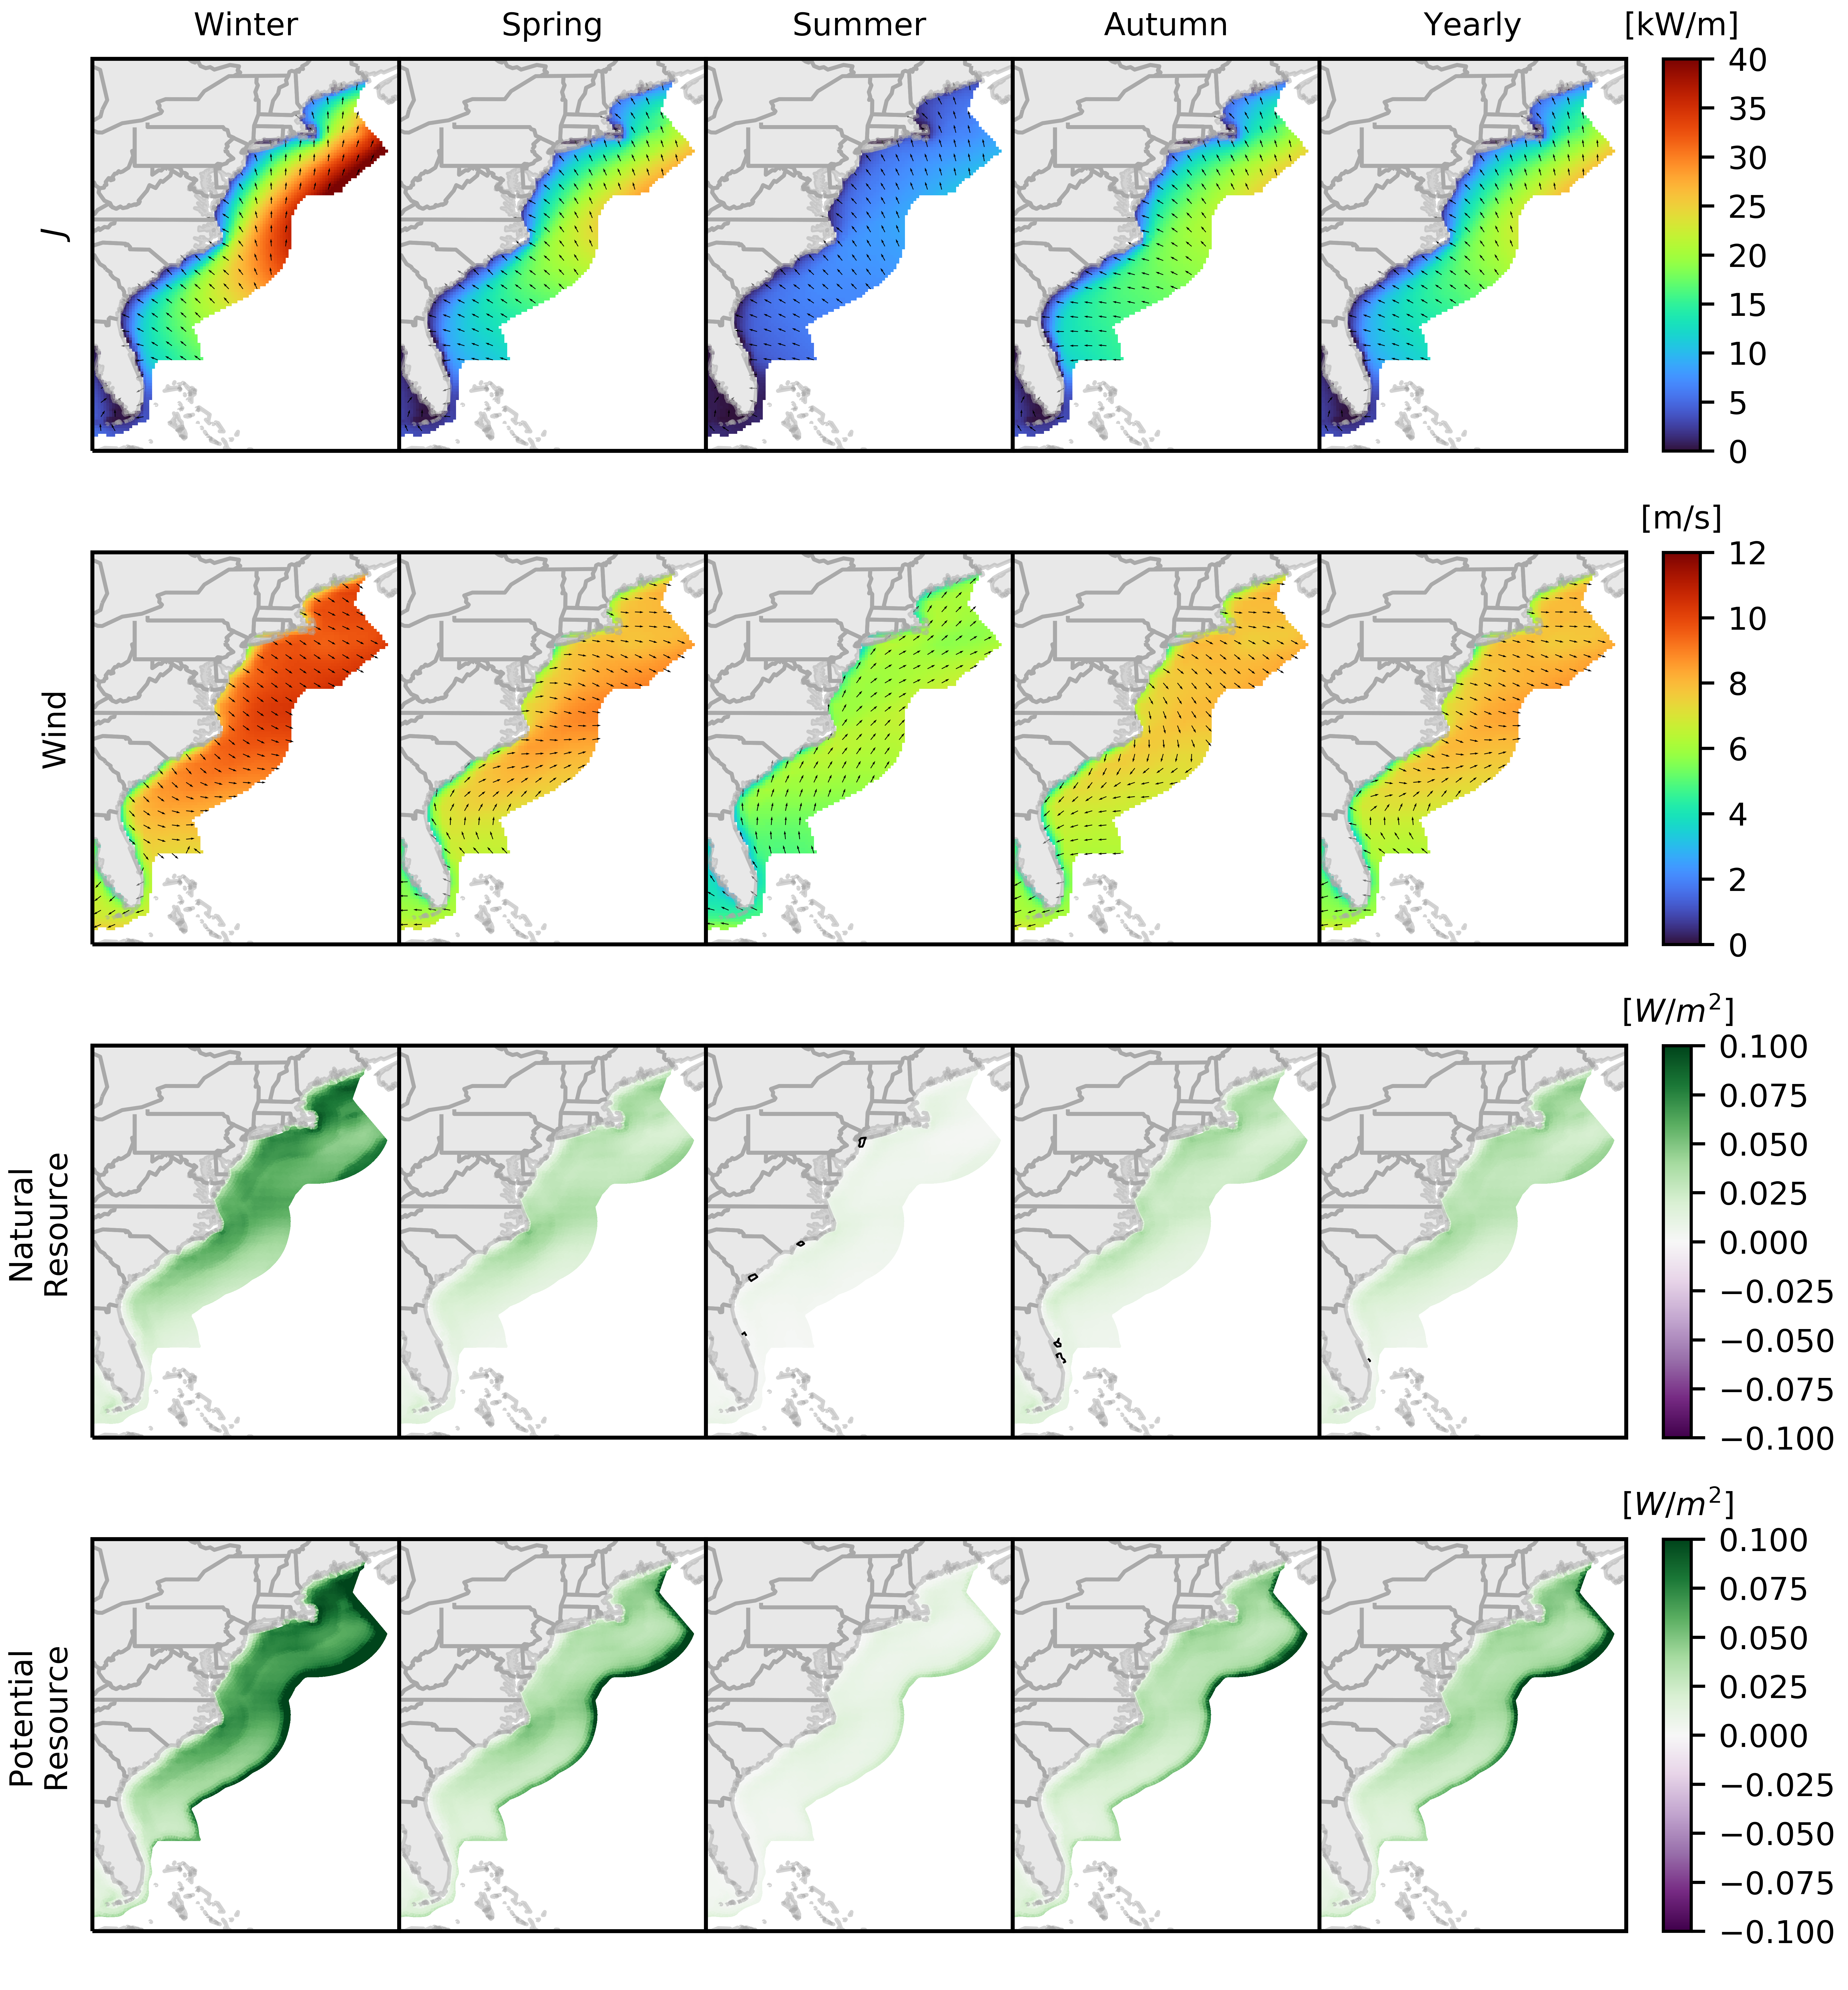
\includegraphics[width=\textwidth]{../fig/at_spatial_seasonal_mag_4.pdf}
%   \caption{Same as \ref{fig:maps-at} for East Coast.}
%   \label{fig:maps-at}
% \end{figure}

\begin{figure}[ht]
  \centering
  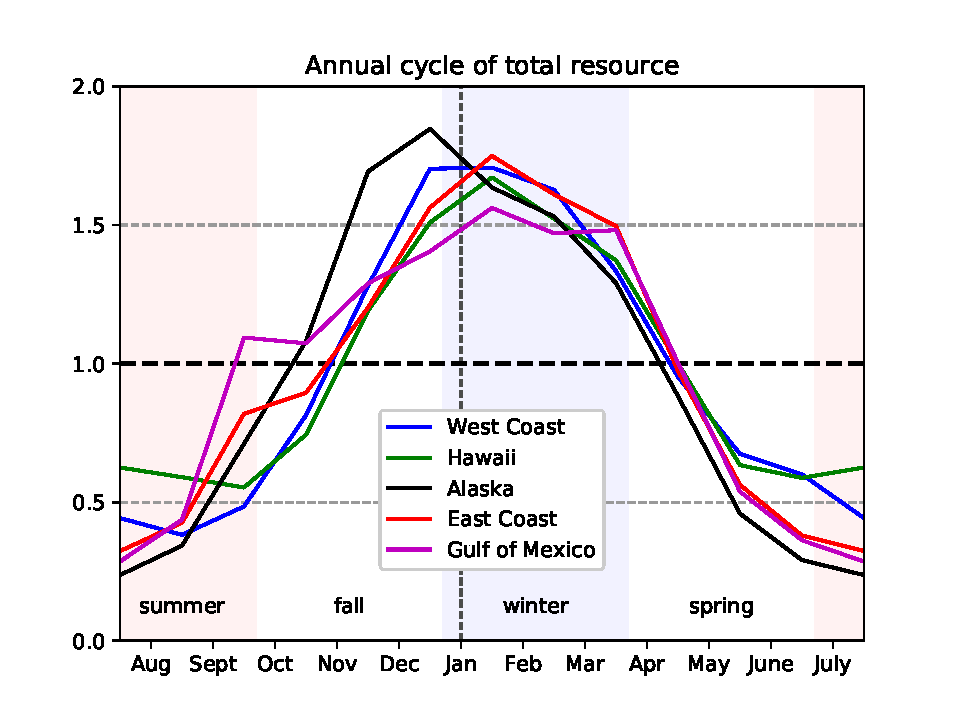
\includegraphics[width=\textwidth]{../fig/AnnualCycle01.pdf}
  \caption[Wave resource annual cycle.]{The annual cycle of the total wave energy resource for several regions, relative to the regional mean.}
  \label{fig:annual-cycle}
\end{figure}


%\begin{figure}[ht]
%  \centering
%  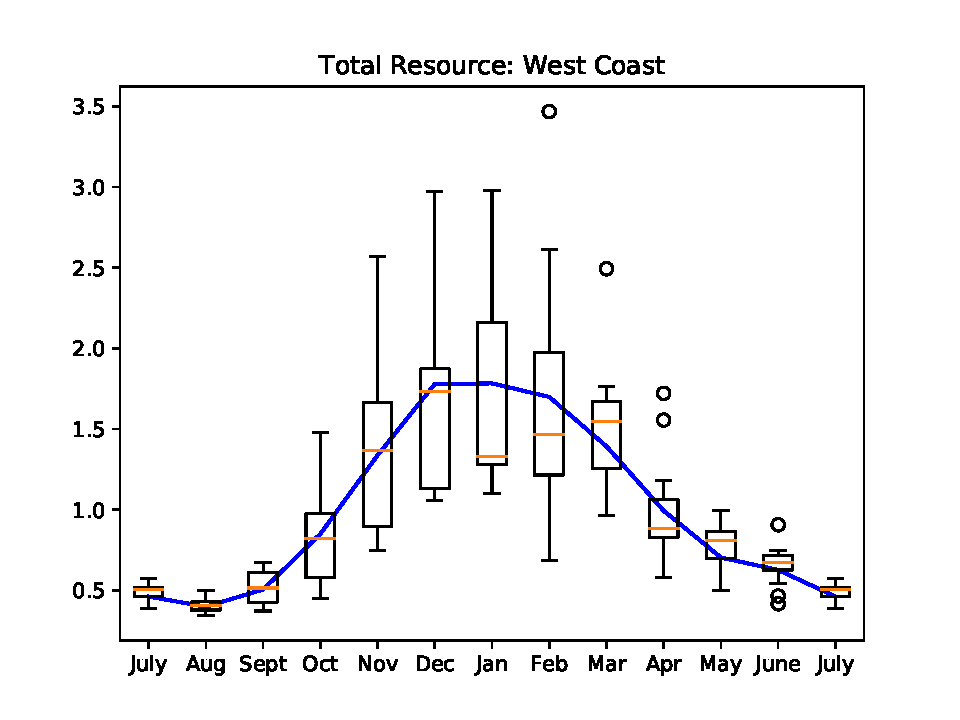
\includegraphics[width=\textwidth]{../fig/AnnualVar01.wc.pdf}
%  \caption[West Coast resource variability.]{Annual and inter-annual variability of the West Coast resource. The thick solid line indicates the mean, and the orange lines and boxes indicate the median and quartiles, respectively. The whiskers extend to the last point within 1.5x of the inter-quartile range, and points beyond this are plotted as open-circles.}
%  \label{fig:wc-variability}
%\end{figure}

\begin{figure}[ht]
  \centering
  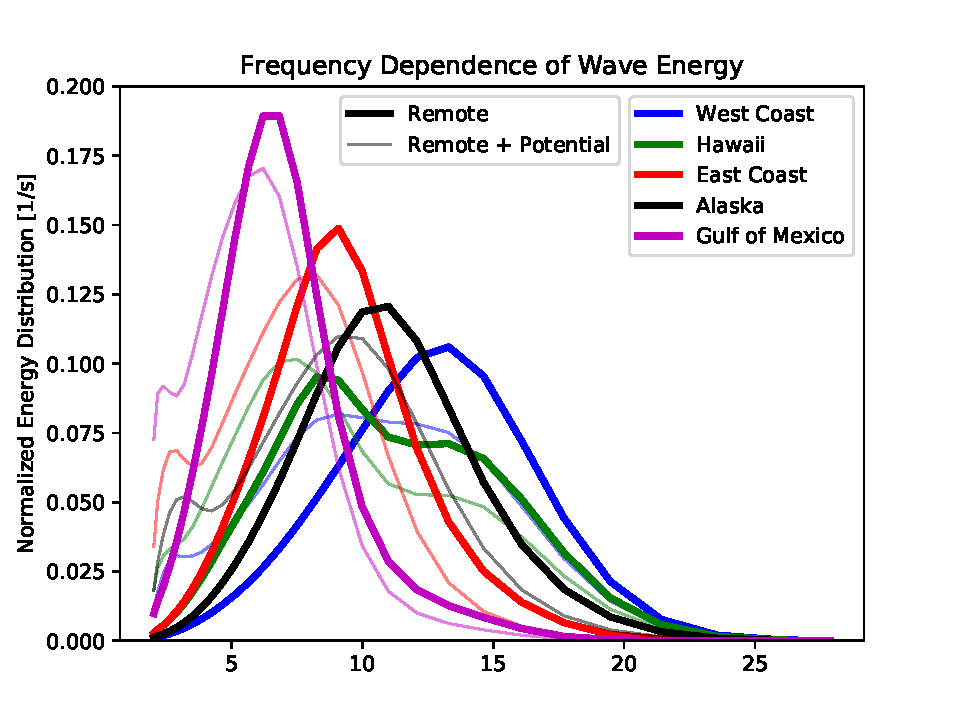
\includegraphics[width=\linewidth]{../fig/TotalResource_Freq02.pdf}
  \caption[Distribution of wave energy vs. wave-period.]{Distribution of wave resource by wave period for each region. Each line represents a spatial average over the entire regional domain. Thick lines indicate the remote resource only, thin lines indicate the sum of the potential and remote resource. Colors are used for each region. Each curve is normalized by its total energy (i.e., the integral of each curve is 1).}
  \label{fig:remote-freq}
\end{figure}

%%% Local Variables:
%%% TeX-master: "wave_res"
%%% End:

\section{Discussion} \label{sec:discussion}

Including the natural or potential local resource in estimates of total theoretical wave energy assessments -- as we propose here -- is a fundamental change in methodology. There are several practical questions about how this energy can be harnessed on both large and small scales. 
Most importantly, we note that the ``potential local'' resource only becomes available when large-scale wave energy extraction becomes economically feasible. Even the ``natural local'' resource doesn't become a significant component of a wave energy projects resource until the size of the project is greater than several thousand square kilometers. As an example, consider fetch limited wave growth under a constant 10 m/s wind in deep water. Following \citet{donelan1980similarity} it will require 50 km of fetch for waves to have an omnidirectional wave power of 1.5 kW/m. 
% \note{Need to check on these numbers.}\textcolor{green}{We can reference the fetch limited wave growth formulae here if that is what you had in mind.} \note{That's exactly what I'm looking for here! Thanks! Can you add that?} Yes

There is also work to be done in understanding how much of the local resource overlaps with the offshore wind resource (i.e., does extracting wave energy -- so that the wave surface is flatter -- reduce or increase the offshore wind resource?). Along these lines, and especially in locations where the seasonality of OSW compliments the wave resource (e.g., as noted in section \ref{sec:results:wc-dist}), it is intriguing to consider the development of projects designed to harness both wave and OSW energy. \textcolor{green}{The proposed methodology is well suited to evaluate this scenario.}

There is also the question of what kinds of devices will efficiently harness this relatively high-frequency energy. Will new device designs be required to harness that energy? If so, will they be economically competitive? Or, will WEC devices of the future be sufficiently broad-banded to extract the local resource and remote resource equally efficiently? 

Harnessing the extra energy in the {\em potential} local resource provides even greater challenges. In particular, tapping into this piece of the wave resource will require extracting large fractions of the remote resource very far from shore, so that their is sufficient fetch for waves to grow and be harnessed by WEC arrays inshore.  

Though these issues exist, we still propose that including the local resource in the total is important for several reasons. First and foremost, it is a real part of the total energy that is contained in the resource, and available for conversion to electricity. Therefore, it falls squarely in the IEC definition of ``theoretical resource''. Second, including it resolves outstanding questions associated with earlier resource assessments (i.e., ``how much energy is available inshore of a chosen boundary?''). This question is especially addressed/resolved by the {\em potential} local resource. And third, including it broadens our understanding of what wave energy is. That is, there is a significant amount of energy at relatively high frequency that could be useful for PBE applications that require relatively small amounts of power. Furthermore, the methodology proposed here -- which has been applied at a regional scale -- can also be applied at the project scale (e.g., down to a single device represented by a small box).
This accuracy at all scales makes it ideally suited for broader adoption by the international community, which will in turn make the assessment of market opportunities more comparable and transparent.

Currently, the IEC Wave Resource Assessment technical specification (TS) focuses on quantifying resource parameters that are important to characterizing the resource across different spatial scales (i.e., three "classes" of resource assessment), but it provides little guidance on how to sum the theoretical resource for a region or site of interest. This is because this technical specification is focused primarily on characterizing the resource for feasibility studies (class 1 and 2) and quantifying the resource for designing projects where technologies are known (class 3). At the feasibility level, omni-directional wave power serves as a useful metric for quantifying the opportunity for wave energy development. When conducting array design, the TS states that ``the effects of the WEC array on wave propagation should be included in the numerical model. Any modifications made to the numerical model to account for the effects of a WEC array shall be documented and justified.'' This is important guidance that effectively accounts for wave directionality, but it is not practical or feasible when performing large-scale theoretical resource assessments for arbitrary devices. Instead, the approach used here skips the complexity of simulating many (thousands to millions or more?) of individual WECs extracting energy, and instead treats the line as a `perfect' array that extracts all of the incoming energy. By using a line-integral (dot-product), we are accounting for the directionality of waves (i.e., the `shadowing effect' of arrays) that is called for in the standards. Thus, the line-integral approach effectively accounting for the `shadowing effect' that is required by the IEC TS, and therefore this approach is consistent with it.

The approach described here may be worthy of consideration for inclusion in the IEC TS because it provides a means of quickly and efficiently estimating the maximum power that could be extracted from a project site. In those cases, the approach is identical to that described here, except that the one-way line-integral should be performed along a boundary enclosing the project site, and the `local resource' is estimated as an area integral over the project site. In general the local resource will most likely be small -- and often negligible (smaller than the uncertainty in the remote resource) -- because the physical dimensions of realistic projects is much smaller than the fetch of typical storms. Nevertheless, computing the local resource is relatively straight-forward so long as the model used has an option for saving the source terms.

\subsection{The potential for wave energy in the U.S.}

\note{Statement about early-stage of WEC tech?}

The U.S. has vast wave energy resources. The West Coast is typically viewed as the premier U.S. market because the resource magnitude and intensity are both high, and the West Coast energy market is large. The west coast theoretical resource (~570 TWh/yr) is equal to about 60\% of electricity consumption by the three coastal states there (CA, OR, WA 2018 total: 943 TWh/yr), which indicates that their is sufficient resource to play a sizable role in the region's energy profile \citep{energyinformationadministrationStateEnergyConsumption2020}.  
\note{I'm getting "570 TWh/yr" as the midpoint in the WC resource. This makes me realize that people will probably want "one number" to point to as the "Theoretical Resource". Should we follow this approach (midpoint between local and potential, plus remote), or just use remote + potential?!}\textcolor{green}{I would rather pick the lower end (remote + local), requires less explanation/justification.}
The fact that the remote wave energy resource here complements the offshore wind resource in several locations, suggests that OSW-wave hybrid projects might have higher annual capacity factors than projects involving one of these technologies alone. The PacWave test site, offshore of central Oregon, has been created to be the first U.S. "grid-connected full-scale test facility", which will provide the opportunity to develop and demonstrate technologies in this world-class ``fully energetic'' resource where winter storms can deliver wave amplitudes greater than 8 meters \citep[e.g.][]{allan_climate_2006}.

Though Alaska has a larger total resource than the West Coast, the majority of this is `stranded'. That is, it is located very far from large populations where markets are large enough to attract projects bigger than a few MW. Still, the wave resource along Alaska's Aleutian chain is sizable, and raises the possibility of the export of Alaska's wave resource if and when large-scale energy storage technologies become sufficiently economical (e.g., liquid fuel storage, batteries, etc.). \textcolor{green}{This energy could also be used in situ, where vessels or scientific instruments can charge their batteries during long transits and exploration.} Could a breakthrough of this kind reignite Alaska's energy-export economy, this time for Alaska's vast renewable energy resources (including wave)? In the shorter-term, the villages along Alaska's coastline -- where energy prices are very high -- represent an opportunity to demonstrate commercial viability before scaling the technology up \cite{alaskaenergyauthority2019PowerCost2020}.

Hawaii possesses a relatively large resource (~430 TWh/yr total, 120 TWh/yr inner-shelf) considering the State's population and electricity consumption (26 TWh/yr), and is an especially attractive early market for wave energy because of the high-energy prices there. 
Wave energy may be particularly valued in Hawaii where space is limited for land-based renewable alternatives; the tourist economy there may especially value WECs with limited surface expression. Together, these factors make Hawaii a likely early-market for wave energy technology. The Navy's Wave Energy Test Site on the north shore of Oahu, is supporting the development and demonstration of technologies for meeting the potential demand \citep{crossEarlyResearchEfforts2015}.

The East Coast and Gulf of Mexico wave resources are modest in comparison to the above regions. Still, it is too early to neglect the potential for wave energy in these regions. As wave technologies continues to mature and if the cost of the technology is low enough, sites and regions previously considered uneconomical may prove to be attractive, especially in markets where energy prices are already high and alternate renewable sources are limited or constrained. \note{I was trying to give a nod to Puerto Rico/USVI here (high energy prices. But, does solar work here? What about OSW? Other ideas GGM?}\textcolor{green}{Small grids such as those in PR/USVI are inherently less stable because you cannot just connect to a neighboring powerplant. Thus  having diversity in the energy mix can help grid stability by compensating when for instance you have a cloudy week. IDK how to say this in an eloquent way.}

\subsection{Predictability of wave energy}
One of the main advantages of wave energy is the idea that it is much more predictable than most other renewable energies. On daily to weekly timescales, wave can be predicted by wave propagation models driven be realtime storm data from ocean basins. On inter-annual timescales, several works have noted a correlation with ENSO fluxuations. Figure \ref{fig:wc-nino} compares the West Coast remote wave resource anomaly (the deviation from the annual mean) to the Oceanic Nino Index (ONI) lagged by 2 months. \cite{nationaloceanicandatmosphericadministrationOceanicNinoIndex2020}.
Here we see a strong correlation between the highest values of the west coast resource and high values of ONI. The fact that the wave resource lags the ONI suggests that the ONI can be used to predict peaks in wave energy. This correlation is likely to be causal because ENSO events are correlated with larger storms in the S. Pacific, which is a major source of wave energy on the U.S. West Coast \cite{andersonClimateIndexOptimized2018, yangCharacteristicsVariabilityNearshore2020,ruggerio_national_2013}. \note{Is ENSO correlated w/ S. Pacific storms?! Did I get that last sentence right?} \texcolor{green}{Yes, the tracks of the storms shift and you get more oblique wave energy. I added Ruggiero 2013 as an extra reference.}
what other kinds of statistical relationships might exist in climate patterns that can be used to maximize wave predictability. \textcolor{green}{At shorter timescales waves are predicted with high accuracy with significant improvements in recent years \citep{cavaleri_wave_2018}. Applications of artificial intelligence has shown promise for accurate prediction of wave height and wave power \citep[e.g.][]{cornejo-bueno_significant_2016}.} This predictability, and the degree to which wave energy compliments other RE sources in certain locations, may become increasingly valuable as electrical grids are powered increasingly by variable renewables \cite{parkinsonIntegratingOceanWave2015}.

\begin{figure}[ht]
  \centering
  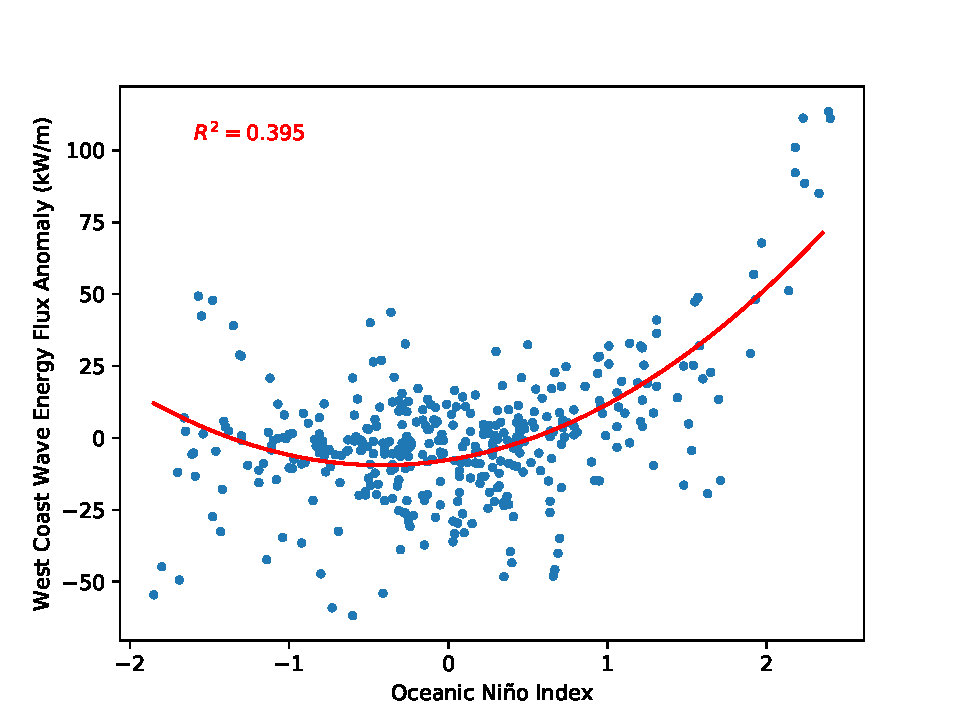
\includegraphics[width=\textwidth]{../fig/ENSO-Comparison.wc.pdf}
  \caption{West Coast wave energy flux anomaly vs. oceanic nino index. The wave energy flux anomaly (annual cycle removed) is averaged along the EEZ boundary, has had a 5-month running average applied, and lags the ONI signal by 2-months.}
  \label{fig:wc-nino}
\end{figure}


\section{Conclusion} \label{sec:conclusion}

We propose a methodology for theoretical wave resource assessment that resolves several outstanding issues with earlier approaches. In particular, this work accounts for wave directionality in order to reduce `double counting', and also includes the energy added to the wave field by local winds. This provides a consistent methodology for accounting for wave energy at national/regional scales. So that policy makers can have a clear understanding of wave energy potential. As other nations/regions adopt the methodology, we will have an apples-to-apples comparison of opportunity, which can inform decision making and investment.

We then apply this methodology to the U.S. EEZ (except for the portion of the EEZ associated with U.S. Pacific Islands Territories), and find that the total U.S. wave energy resource is greater than 3,300 TWh/yr.
\note{We need to decide which `one number' we're going to use here.}
This is an increase of ~25\% compared to earlier DOE wave resource assessments, and is due to the combination of extending the resource area to the edge of the EEZ and incorporating the local resource. The `inner shelf' resource also increases from a total of ~1600 TWh/yr in EPRI 2011 to 1800 TWh/yr here. \note{Most of the increase is in AK. Why?! ... The 'inner shelf' remote resource is > than the EEZ remote resource. Is this just because the contour is longer? Is it worth discussing this nuance in RESULTS or DISCUSSION?}

A detailed assessment of the ``technical resource potential'', which accounts for the efficiency and array design of existing technologies is left for future work. Furthermore, an assessment of the ``practical resource'' is a greater challenge because it requires accounting for regional permitting details, ocean-planning designations, and competing uses by other ocean stakeholders.

We encourage he IEC wave resource assessment team to consider adopting pieces of this methodology in the ``reconaissance'' level assessments in order to promote the use of regional resource assessment that can be compared. Furthermore, the methods proposed here could also be of use to project developers in identifying the maximum resource potential of a project site. \note{Need to think about how to say this more tactfully.}


%%% Local Variables:
%%% TeX-master: "wave_res"
%%% End:


%\appendix

%\section{On the details of estimating the remote resource} \label{appendix:delta}

\subsection{The importance of accounting for wave directionality} \label{appendix:directionality}

\note{Add a short intro about the importance of wave directionality here? (OWP is valuable, but `unit circle' method is bunk.)}

As the National Academy review points out, estimates of $R_r$ must account for wave directionity in order to avoid double-counting. For example, when a wave with energy density of $1 \unit{kW/m}$ crosses a 1 km integration contour segment with its wave crests parallel to the segment, the total power is 1MW (upper row of Figure \ref{fig:directionality}). Likewise, when that same 1-km wide wave crosses a contour-segment with its wave crests at an angle to the integration contour, the total energy contained in the wave is still only 1 MW. The directionality coefficient corrects for fact that the length of the contour segment is longer to capture the whole 1-km wave at an angle (3 km in lower row of Figure \ref{fig:directionality}, where $\theta = 70.5 \unit{degrees}$). In the `unit circle' method described in the 2011 resource assessment $\delta$ is taken to be $1$ in all cases (directionality is neglected), which for the wave depicted in the lower row of Figure \ref{fig:directionality} gives an estimate of 3 MW crossing the contour. This is clearly incorrect since the 1-km wide wave only contains 1 MW of power, and demonstrates the importance of accounting for directionality.

\begin{figure}[ht]
    \centering
    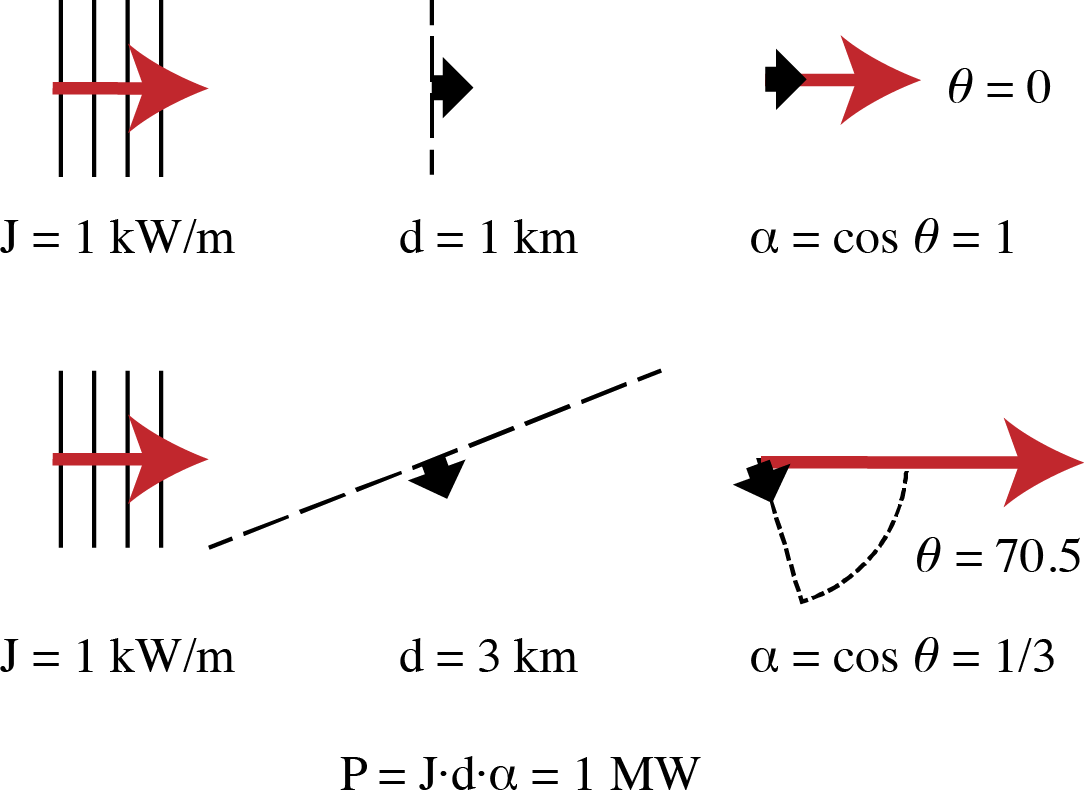
\includegraphics[width=0.6 \linewidth]{../diagram/Dot-Product_Schematic01.png}
    \caption{A diagram depicting the importance of accounting for wave directionality. The upper sequence depcits a scenario where wave crests are parallel to the integration contour ($\delta = 1$), and the lower row is a scenario where wave crests are oblique to the contour ($\delta = 1/3$). \note{I need to change the $\alpha$'s in this figure to $\delta$'s.}}
    \label{fig:directionality}
\end{figure}

One of the main reasons there has been confusion about this topic is due to the fact that many types of WECs are agnostic to the direction that wave energy arrives from (Figure \ref{fig:omni-dir}A, and \cite{EPRIwaveresource2011} ). That is, all other things being equal (wave height, period, etc.), these `omnidirectional WECs' generate the same amount of power regardless of the direction that wave energy arrives from. For a single WEC of this type, it is possible to obtain an estimate of power output by simply multiplying the device's capture-width by the omnidirectional wave power. However, when you start arranging many of these WECs together in an array where their spacing is close enough to capture all of the incident energy, then they begin to shadow one-another in a way that depends on wave direction and array-layout (i.e., in a similar manner to how wind turbine wakes reduce the performance of down-wind turbines). Accurately modeling arrays of devices is technically challenging, but the point here is that directionality matters for WEC arrays and obviously you can't get more energy out of the waves than exists in them \note{add some WEC-sim array citations here?}. For the purposes of theoretical wave resource assessment then — instead of attempting to model arrays of devices that extract all of the energy in the wave-field — we simply draw an integration contour and assume that we can extract all of the energy that crosses it (i.e., by properly accounting for directionality). 

\begin{figure}[ht]
    \centering
    \fbox{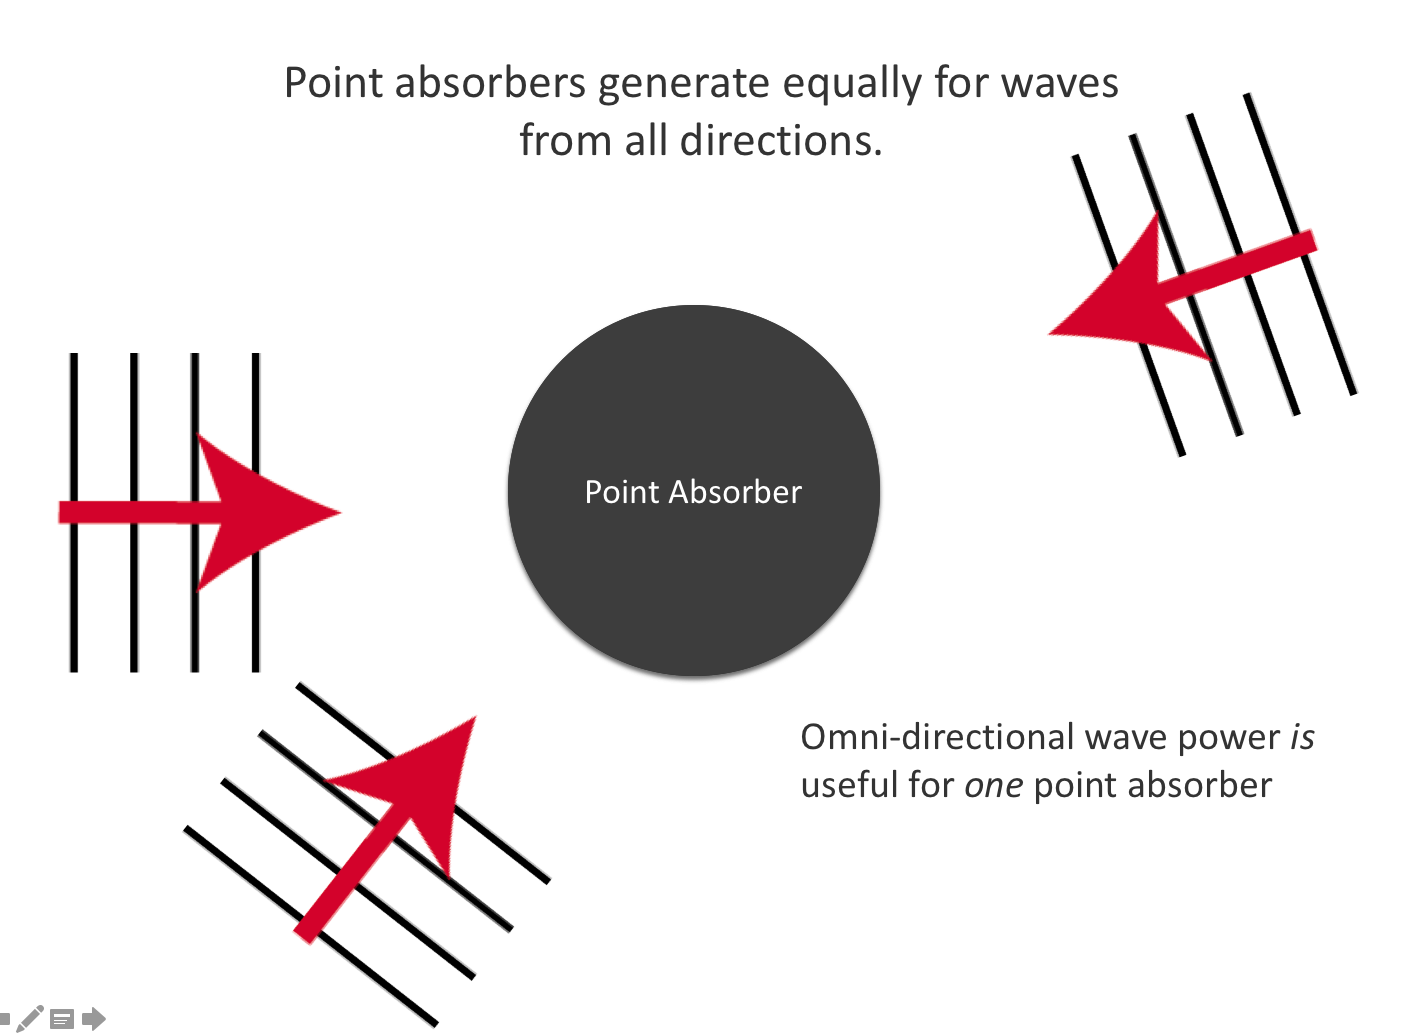
\includegraphics[width=0.3\linewidth]{../diagram/omni-dir01}}
    \fbox{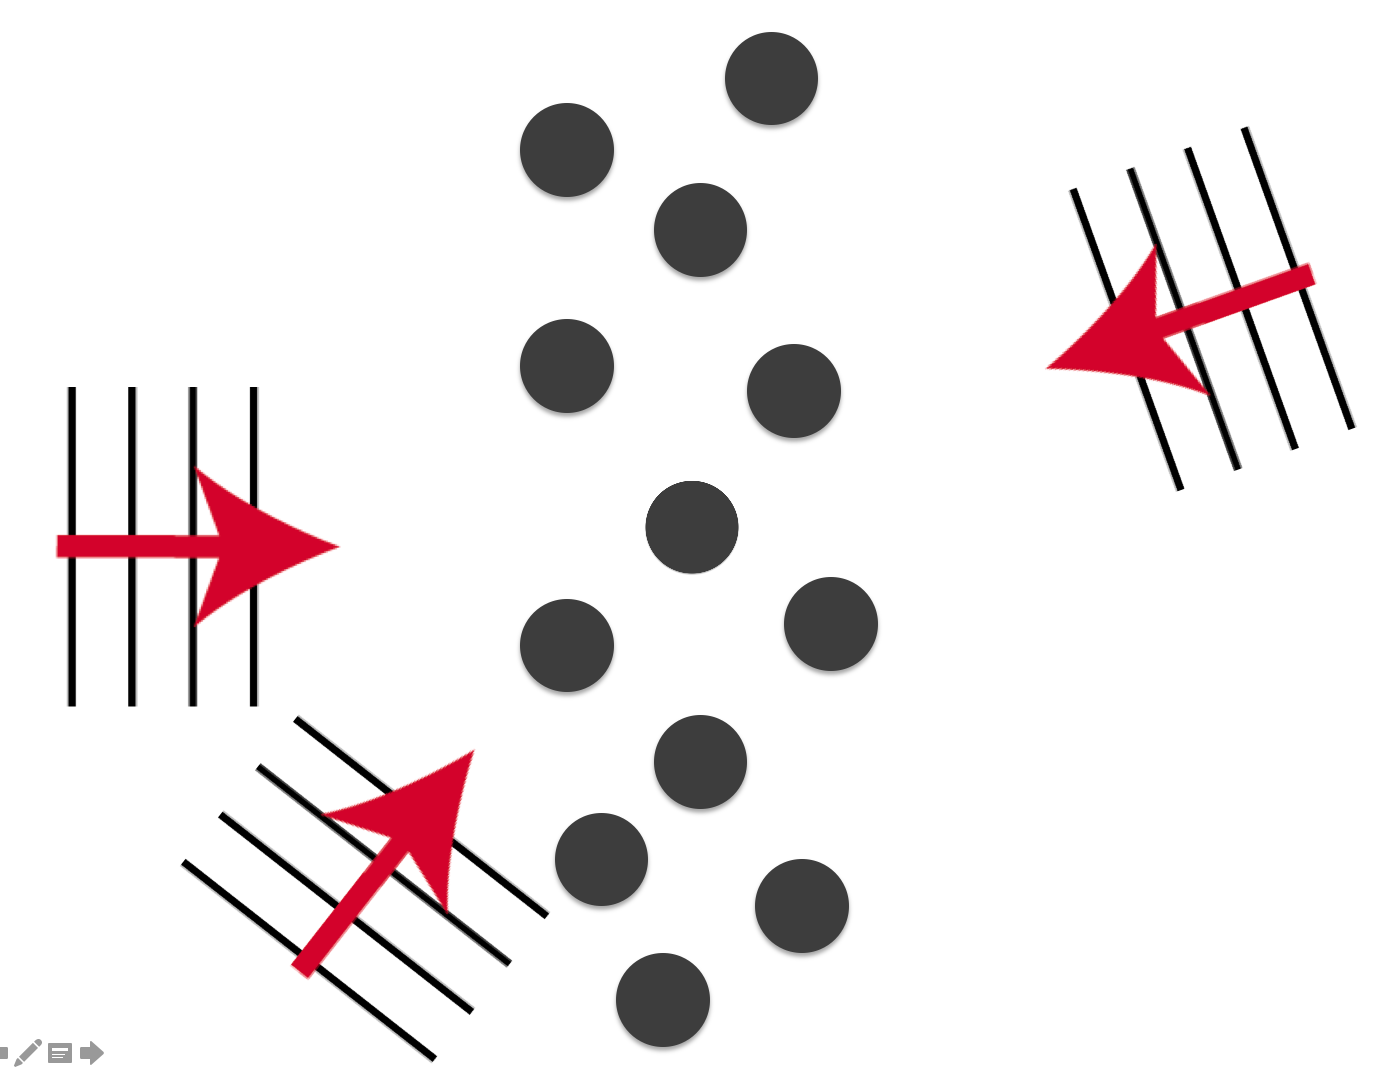
\includegraphics[width=0.3\linewidth]{../diagram/omni-dir02}}
    \fbox{
\includegraphics[width=0.3\linewidth]{../diagram/omni-dir03}}
    \caption{A) A ``point absorber'' type omni-directional WEC is denoted as a black circle. B) Though a single ``point absorber'' does not care about wave-direction, an array of such devices does because individual devices shadow one-another depending on wave direction. C) Shadowing is indicated explicitly in this case where the array is a line of ``point absorbers' spaced close enough to capture all incoming energy.\note{These figures are place-holders for now. }}
    \label{fig:omni-dir}
\end{figure}

\subsection{A detailed discussion of the `one-way' approach to estimating the remote resource}

The one-way approach to estimating $R_r$ deserves some explanation because it deviates from the traditional definition of a line-integral. In a traditional line-integral the directionality coefficient is simply:
\begin{align}
    \delta_{*} = \cos(\theta_n - \theta)
    \label{eqn:trad-def}
\end{align}
The primary problem with this definition for the purposes of wave resource assessment is that waves that propagate away from the shoreline of interest ($|\theta_n - \theta|>90$) are subtracted from the resource total. This motivates consideration of two alternate definitions of $\delta$. First, a `bi-directional' case:
\begin{align}
    \delta_2 = |\delta_{*}|
    \label{eqn:2way-def}
\end{align}
and the one-way case:
\begin{align}
    \delta_1 = 
    \begin{cases}
     \delta_* & \mathrm{for\ }|\theta_n - \theta|<90^\circ \\
    0 & \mathrm{otherwise}.       
    \end{cases}
    \label{eqn:1way-def}
\end{align}
In weighing the pros/cons of these definitions of $\delta$ it is important to understand that wave resource assessments are typically based on models that do not extract wave energy when it encounters the integration contour of interest (e.g., $\leez$). That is, wave energy that propagates across the integration contour at one location might propagate across it again at another location, and there is typically no way to `track' waves (i.e., wave energy) within these models.
This means that both of the definitions of $\delta$ in \eqref{eqn:2way-def} and \eqref{eqn:1way-def} will `double-count' waves that criss-cross back-and-forth across the integration countour ($\delta_2$ to a larger degree). This can occur for waves that travel straight across a zig-zagging integration contour, or for waves that zig-zag along a straight contour. 

\begin{figure}[ht]
    \centering
    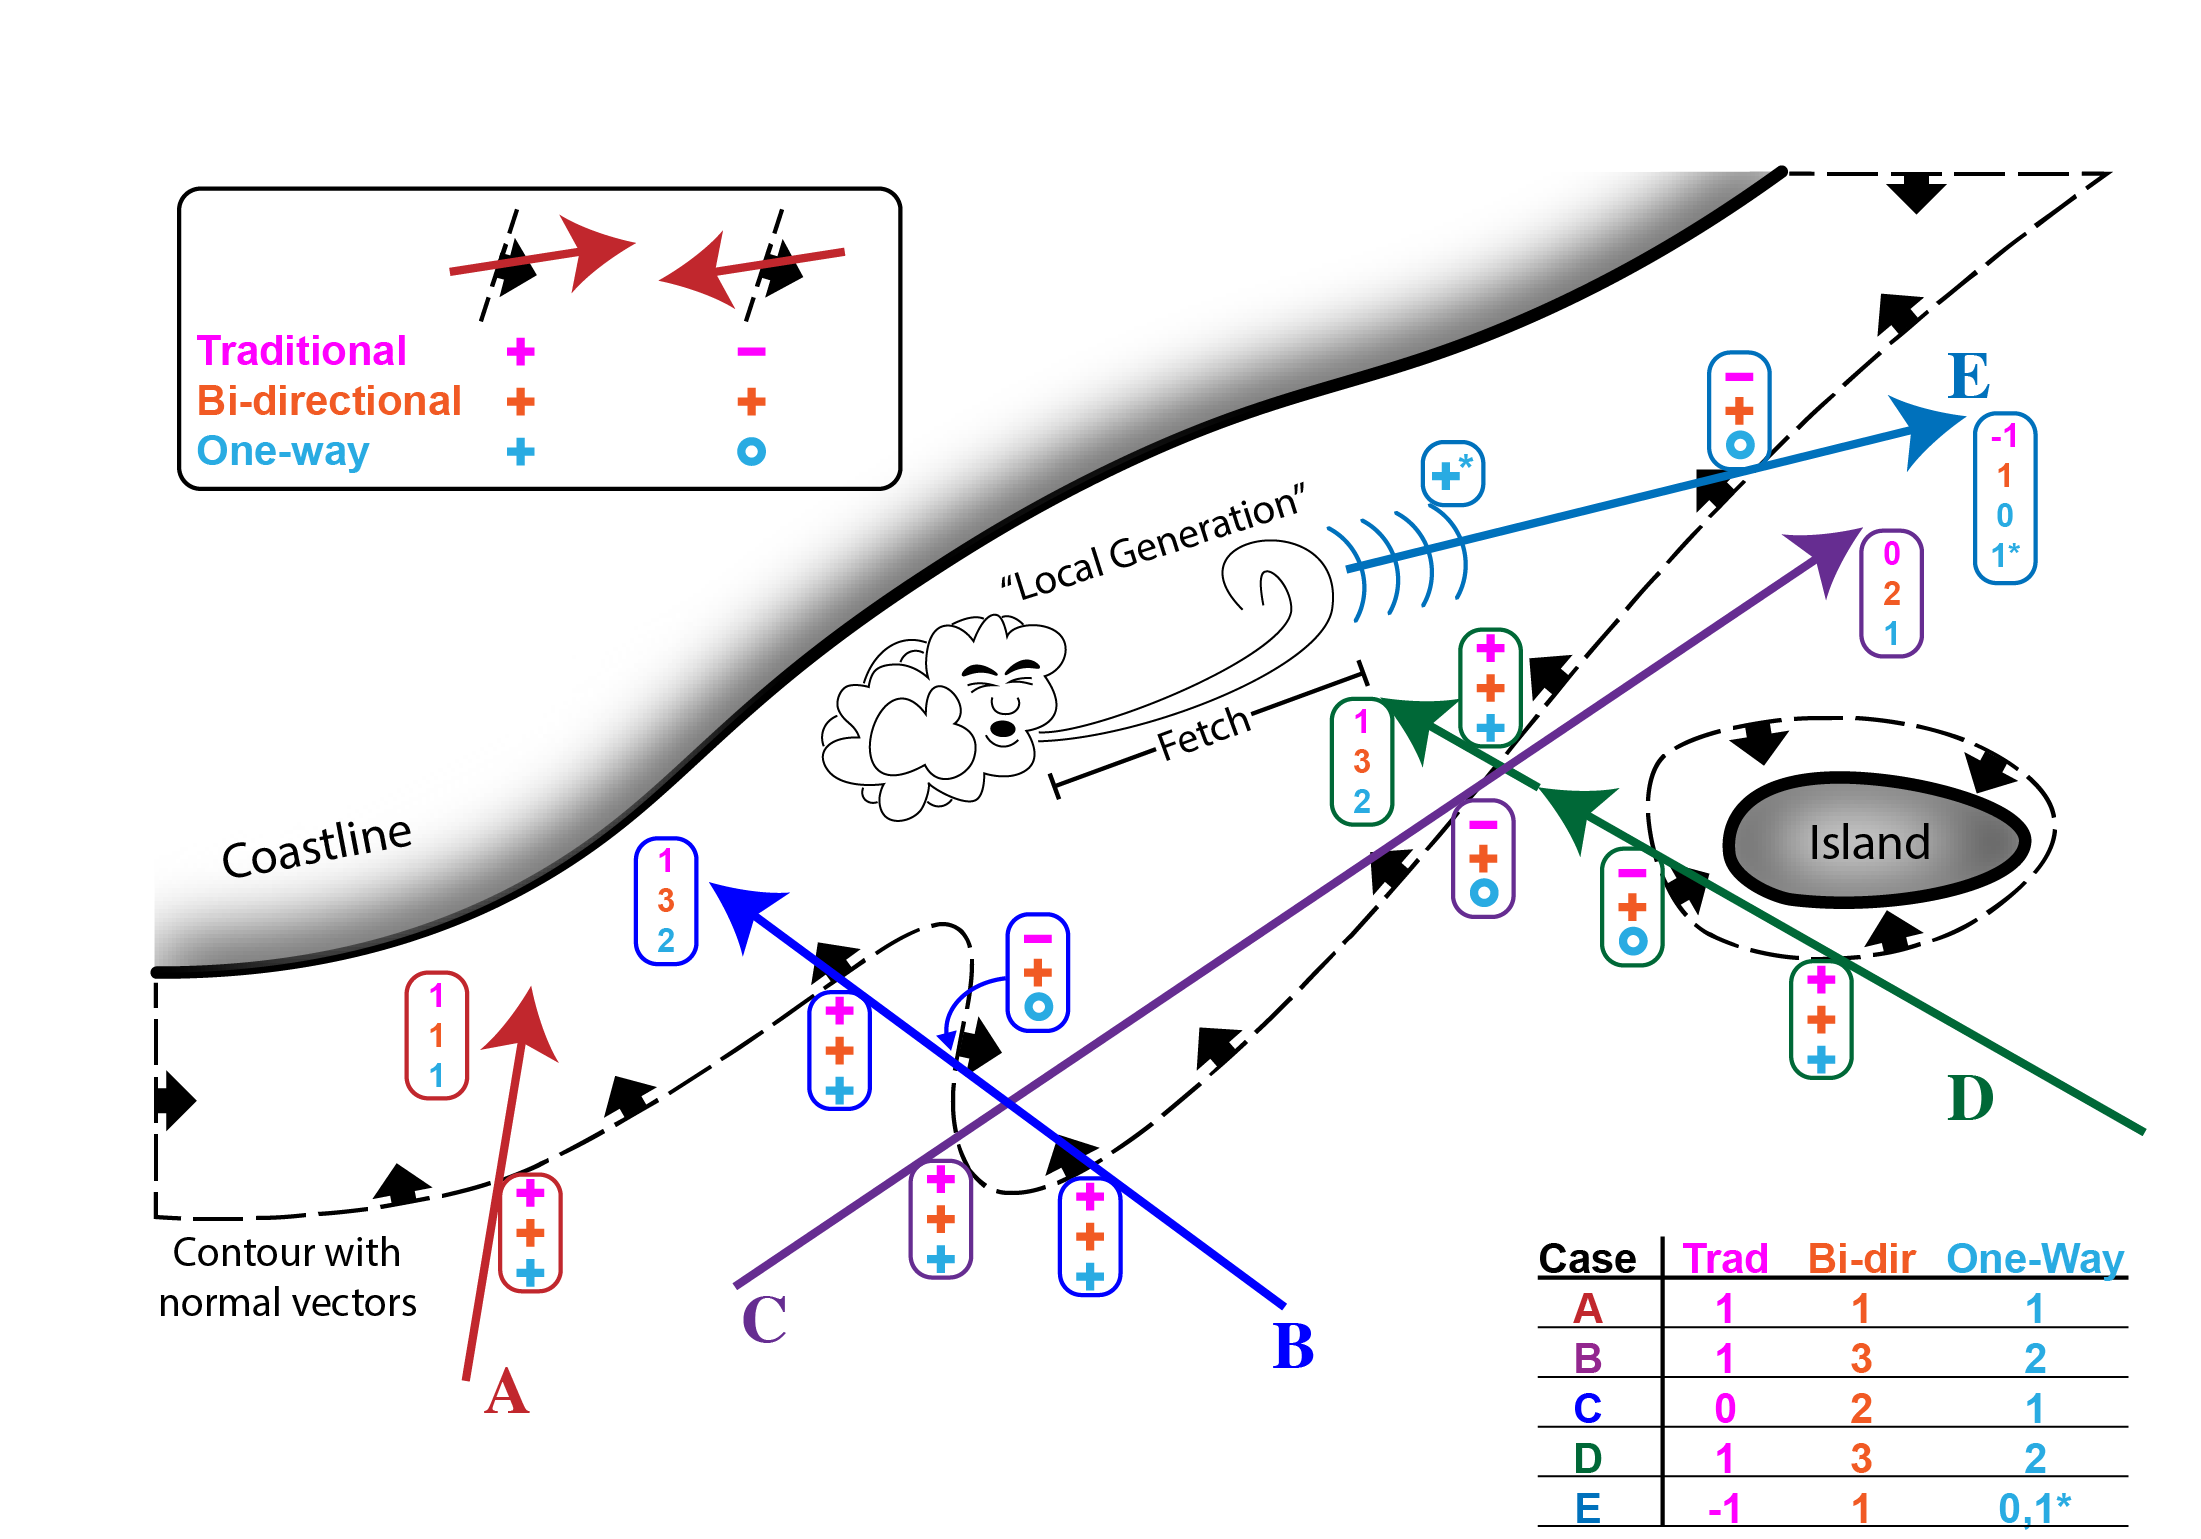
\includegraphics[width=\linewidth]{../diagram/Schematic-Seq01FINAL.png}
    \caption{A diagram depicting different cases of waves (color arrows) crossing an arbitrary integration contour (black dashed line). Black arrows along the contour indicate the contour-normal direction. The upper-left legend — and the boxes along the arrows' lengths — indicate whether energy is added to, subtracted from, or not included in the total depending on the summation method (pink: traditional, orange: bi-directional, cyan: one-way) and direction of wave crossing relative to contour. Boxes at the tip of each arrow indicate the number of times each wave was counted using each method, and the table at lower-right summarizes the totals. A `blowing cloud' image indicates the generation of `local waves' over the region bounded by the integration contour. \note{Need to add a row $E^\dagger$}}
    \label{fig:one-way-diagram}
\end{figure}

Figure \ref{fig:one-way-diagram} provides a schematic of several distinct cases of wave energy (color arrows) propagating across an arbitrary integration contour (black dashed line). Arrow `A' (red) indicates the simplest case of a wave train crossing the contour once before dissipating at the coastline. In this case, all three definitions of $\delta$ give the same correct result of counting this wave exactly once. Arrow `B' (blue) is the case where a wave crosses a zig-zagging countour several times, and shows that $\delta_1$ and $\delta_2$ double-count and triple-count this wave. Arrow `C' (purple) is a case where a wave propagates into and out-of the integration boundary, demonstrating that the $\delta = \delta_*$ does not count this wave, $\delta_1$ counts it once, and $\delta_2$ double-counts it. Arrow `D' (green) is the case of a wave propagating through an island's contour before entering the mainland contour, with essentially the same result as wave `B'. It is also interesting to consider the case where wave `D' does not enter the mainland contour (i.e., if the island is far from shore), in which case the results are the same as wave C.

Finally, this brings us to case `E' where a wave is generated inshore of the boundary and propagates offshore. In this case the wave's energy is subtracted from the total for the traditional case, not counted for the one-way case, and added once (correctly) for the bi-directional method. Note that this is the only case—other than simple case (A)—where the bidirectional method delivers the correct result. When the one-way method is used in conjunction with the local resource method, this waves' energy is included in the total.
When the local resource is added to the numbers in row E, this wave's energy is counted again, which yields row E$^\dagger$.

Importantly, the table in Figure \ref{fig:one-way-diagram} shows that none of the methods defined by the definitions of $\delta$ deliver an accurate estimate of the wave resource for all possible wave paths and integration contours. The only way to avoid double-counting completely is to extract wave energy at the integration contour so that it does not propagate to a different point on the contour where it could be double-counted (or subtracted, depending on the choice of $\delta$). This approach, however, is technically challenging and reduces the flexibility of data analysis (i.e., simulations must be run for each integration contour the user wishes to investigate).

Instead, it is worthwhile to note that $\delta_*$ will provides a lower-bound estimate of $R_r$ (all values are $\le 1$ in the table on Figure \ref{fig:one-way-diagram}), the bidirectional method provides an upper-bound (values $\ge 1$), and the one-way method provides a `best-estimate'. The one-way method is especially accurate when the local waves are accounted for independently (i.e., as $R_l$), as indicated by the `$1^*$' in Figure \ref{fig:one-way-diagram}. Also, the one-way method only over-estimates when waves criss-cross into the boundary multiple times. As long as integration contours are not zig-zagged and assuming waves do not themselves zig-zag across the boundary (i.e., assuming wave turning is not a major issue at the scale and water depth of the integration contour), then the one-way method in conjunction with $R_l$, is a reasonably accurate estimate of the total theoretical resource ($R_t$).

\note{Should we include a table of the different estimates of $R_r$ (e.g., for the west coast) using different definitions of $\delta$?}


%%% Local Variables:
%%% TeX-master: "wave_res"
%%% End:

%\section{Comparing wave flux divergence to source term area integral}\label{appendix:flux-vs-area}

\note{GGM: Do you want to put some of your method comparison here?}


\clearpage

\bibliographystyle{elsarticle-num-names}
\bibliography{refs,refs_GGM}


\end{document}
